\documentclass[twoside]{book}

% Packages required by doxygen
\usepackage{calc}
\usepackage{doxygen}
\usepackage{graphicx}
\usepackage[utf8]{inputenc}
\usepackage{makeidx}
\usepackage{multicol}
\usepackage{multirow}
\usepackage{textcomp}
\usepackage[table]{xcolor}

% Font selection
\usepackage[T1]{fontenc}
\usepackage{mathptmx}
\usepackage[scaled=.90]{helvet}
\usepackage{courier}
\usepackage{amssymb}
\usepackage{sectsty}
\renewcommand{\familydefault}{\sfdefault}
\allsectionsfont{%
  \fontseries{bc}\selectfont%
  \color{darkgray}%
}
\renewcommand{\DoxyLabelFont}{%
  \fontseries{bc}\selectfont%
  \color{darkgray}%
}

% Page & text layout
\usepackage{geometry}
\geometry{%
  a4paper,%
  top=2.5cm,%
  bottom=2.5cm,%
  left=2.5cm,%
  right=2.5cm%
}
\tolerance=750
\hfuzz=15pt
\hbadness=750
\setlength{\emergencystretch}{15pt}
\setlength{\parindent}{0cm}
\setlength{\parskip}{0.2cm}
\makeatletter
\renewcommand{\paragraph}{%
  \@startsection{paragraph}{4}{0ex}{-1.0ex}{1.0ex}{%
    \normalfont\normalsize\bfseries\SS@parafont%
  }%
}
\renewcommand{\subparagraph}{%
  \@startsection{subparagraph}{5}{0ex}{-1.0ex}{1.0ex}{%
    \normalfont\normalsize\bfseries\SS@subparafont%
  }%
}
\makeatother

% Headers & footers
\usepackage{fancyhdr}
\pagestyle{fancyplain}
\fancyhead[LE]{\fancyplain{}{\bfseries\thepage}}
\fancyhead[CE]{\fancyplain{}{}}
\fancyhead[RE]{\fancyplain{}{\bfseries\leftmark}}
\fancyhead[LO]{\fancyplain{}{\bfseries\rightmark}}
\fancyhead[CO]{\fancyplain{}{}}
\fancyhead[RO]{\fancyplain{}{\bfseries\thepage}}
\fancyfoot[LE]{\fancyplain{}{}}
\fancyfoot[CE]{\fancyplain{}{}}
\fancyfoot[RE]{\fancyplain{}{\bfseries\scriptsize Generated on Mon Feb 22 2016 00\-:12\-:39 for Multimedia\-Server by Doxygen }}
\fancyfoot[LO]{\fancyplain{}{\bfseries\scriptsize Generated on Mon Feb 22 2016 00\-:12\-:39 for Multimedia\-Server by Doxygen }}
\fancyfoot[CO]{\fancyplain{}{}}
\fancyfoot[RO]{\fancyplain{}{}}
\renewcommand{\footrulewidth}{0.4pt}
\renewcommand{\chaptermark}[1]{%
  \markboth{#1}{}%
}
\renewcommand{\sectionmark}[1]{%
  \markright{\thesection\ #1}%
}

% Indices & bibliography
\usepackage{natbib}
\usepackage[titles]{tocloft}
\setcounter{tocdepth}{3}
\setcounter{secnumdepth}{5}
\makeindex

% Hyperlinks (required, but should be loaded last)
\usepackage{ifpdf}
\ifpdf
  \usepackage[pdftex,pagebackref=true]{hyperref}
\else
  \usepackage[ps2pdf,pagebackref=true]{hyperref}
\fi
\hypersetup{%
  colorlinks=true,%
  linkcolor=blue,%
  citecolor=blue,%
  unicode%
}

% Custom commands
\newcommand{\clearemptydoublepage}{%
  \newpage{\pagestyle{empty}\cleardoublepage}%
}


%===== C O N T E N T S =====

\begin{document}

% Titlepage & ToC
\hypersetup{pageanchor=false}
\pagenumbering{roman}
\begin{titlepage}
\vspace*{7cm}
\begin{center}%
{\Large Multimedia\-Server }\\
\vspace*{1cm}
{\large Generated by Doxygen 1.8.6}\\
\vspace*{0.5cm}
{\small Mon Feb 22 2016 00:12:39}\\
\end{center}
\end{titlepage}
\clearemptydoublepage
\tableofcontents
\clearemptydoublepage
\pagenumbering{arabic}
\hypersetup{pageanchor=true}

%--- Begin generated contents ---
\chapter{Hierarchical Index}
\section{Class Hierarchy}
This inheritance list is sorted roughly, but not completely, alphabetically\-:\begin{DoxyCompactList}
\item \contentsline{section}{T\-C\-P\-Server\-:\-:Callback}{\pageref{class_t_c_p_server_1_1_callback}}{}
\begin{DoxyCompactList}
\item \contentsline{section}{T\-C\-P\-Server\-:\-:Callback\-Impl$<$ T $>$}{\pageref{class_t_c_p_server_1_1_callback_impl}}{}
\end{DoxyCompactList}
\item \contentsline{section}{Factory}{\pageref{class_factory}}{}
\item \contentsline{section}{Input\-Buffer}{\pageref{struct_input_buffer}}{}
\item list\begin{DoxyCompactList}
\item \contentsline{section}{Group$<$ T $>$}{\pageref{class_group}}{}
\end{DoxyCompactList}
\item \contentsline{section}{T\-C\-P\-Server\-:\-:Lock}{\pageref{class_t_c_p_server_1_1_lock}}{}
\item \contentsline{section}{Multimedia}{\pageref{class_multimedia}}{}
\begin{DoxyCompactList}
\item \contentsline{section}{Group$<$ T $>$}{\pageref{class_group}}{}
\item \contentsline{section}{Photo}{\pageref{class_photo}}{}
\item \contentsline{section}{Video}{\pageref{class_video}}{}
\begin{DoxyCompactList}
\item \contentsline{section}{Film}{\pageref{class_film}}{}
\end{DoxyCompactList}
\end{DoxyCompactList}
\item \contentsline{section}{Process\-Request}{\pageref{class_process_request}}{}
\item \contentsline{section}{Server\-Socket}{\pageref{class_server_socket}}{}
\item \contentsline{section}{Socket}{\pageref{class_socket}}{}
\item \contentsline{section}{Socket\-Buffer}{\pageref{class_socket_buffer}}{}
\begin{DoxyCompactList}
\item \contentsline{section}{T\-C\-P\-Server\-:\-:Cnx}{\pageref{class_t_c_p_server_1_1_cnx}}{}
\end{DoxyCompactList}
\item \contentsline{section}{T\-C\-P\-Server}{\pageref{class_t_c_p_server}}{}
\end{DoxyCompactList}

\chapter{Class Index}
\section{Class List}
Here are the classes, structs, unions and interfaces with brief descriptions\-:\begin{DoxyCompactList}
\item\contentsline{section}{\hyperlink{class_t_c_p_server_1_1_callback}{T\-C\-P\-Server\-::\-Callback} }{\pageref{class_t_c_p_server_1_1_callback}}{}
\item\contentsline{section}{\hyperlink{class_t_c_p_server_1_1_callback_impl}{T\-C\-P\-Server\-::\-Callback\-Impl$<$ T $>$} }{\pageref{class_t_c_p_server_1_1_callback_impl}}{}
\item\contentsline{section}{\hyperlink{class_t_c_p_server_1_1_cnx}{T\-C\-P\-Server\-::\-Cnx} \\*Connection with a given client }{\pageref{class_t_c_p_server_1_1_cnx}}{}
\item\contentsline{section}{\hyperlink{class_factory}{Factory} }{\pageref{class_factory}}{}
\item\contentsline{section}{\hyperlink{class_film}{Film} }{\pageref{class_film}}{}
\item\contentsline{section}{\hyperlink{class_group}{Group$<$ T $>$} }{\pageref{class_group}}{}
\item\contentsline{section}{\hyperlink{struct_input_buffer}{Input\-Buffer} }{\pageref{struct_input_buffer}}{}
\item\contentsline{section}{\hyperlink{class_t_c_p_server_1_1_lock}{T\-C\-P\-Server\-::\-Lock} \\*Locks the server in read mode or in write mode. In order to avoid concurrency problems between threads, the callback method that processes requests should instantiate a \hyperlink{class_t_c_p_server_1_1_lock}{Lock} object in the stack. The \hyperlink{class_t_c_p_server_1_1_lock}{Lock} must be instantiated in write mode if the request changes data, or in read mode otherwise. A write lock blocks all other locks (hence, all other threads) until the callback method that issued the write lock returns }{\pageref{class_t_c_p_server_1_1_lock}}{}
\item\contentsline{section}{\hyperlink{class_multimedia}{Multimedia} }{\pageref{class_multimedia}}{}
\item\contentsline{section}{\hyperlink{class_photo}{Photo} }{\pageref{class_photo}}{}
\item\contentsline{section}{\hyperlink{class_process_request}{Process\-Request} }{\pageref{class_process_request}}{}
\item\contentsline{section}{\hyperlink{class_server_socket}{Server\-Socket} \\*T\-C\-P/\-I\-P \hyperlink{class_socket}{Socket} Server. This class encapsulates a T\-C\-P/\-I\-P socket server. A\-F\-\_\-\-I\-N\-E\-T connections following the I\-Pv4 Internet protocol are supported }{\pageref{class_server_socket}}{}
\item\contentsline{section}{\hyperlink{class_socket}{Socket} \\*T\-C\-P/\-I\-P or U\-D\-P/\-Datagram \hyperlink{class_socket}{Socket}. This class encapsulates a T\-C\-P/\-I\-P or U\-D\-P/\-Datagram socket. A\-F\-\_\-\-I\-N\-E\-T connections following the I\-Pv4 Internet protocol are supported }{\pageref{class_socket}}{}
\item\contentsline{section}{\hyperlink{class_socket_buffer}{Socket\-Buffer} \\*Class for exchanging text strings between T\-C\-P/\-I\-P sockets. T\-C\-P/\-I\-P connected sockets do not preserve record boundaries. Messages can be split or merged so that one call to \hyperlink{class_socket_a9275eacdb64056a53cf4b9cf54cd2f1a}{Socket\-::send()} on the sending side does not necessarily correspond to one call to \hyperlink{class_socket_aa5e98b6f2c4e26fcf90d71c8386fc09d}{Socket\-::receive()} on the receiving side }{\pageref{class_socket_buffer}}{}
\item\contentsline{section}{\hyperlink{class_t_c_p_server}{T\-C\-P\-Server} \\*T\-C\-P/\-I\-P I\-Pv4 server. The server supports T\-C\-P/\-I\-P A\-F\-\_\-\-I\-N\-E\-T connections (following the I\-Pv4 Internet protocol) with multiple clients. One thread is used per client }{\pageref{class_t_c_p_server}}{}
\item\contentsline{section}{\hyperlink{class_video}{Video} }{\pageref{class_video}}{}
\end{DoxyCompactList}

\chapter{Class Documentation}
\hypertarget{class_t_c_p_server_1_1_callback}{\section{T\-C\-P\-Server\-:\-:Callback Class Reference}
\label{class_t_c_p_server_1_1_callback}\index{T\-C\-P\-Server\-::\-Callback@{T\-C\-P\-Server\-::\-Callback}}
}
Inheritance diagram for T\-C\-P\-Server\-:\-:Callback\-:\begin{figure}[H]
\begin{center}
\leavevmode
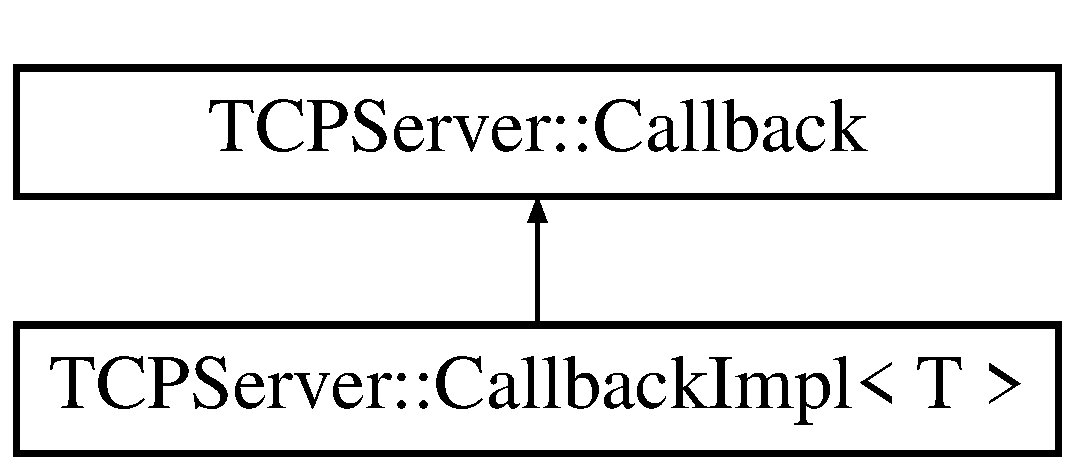
\includegraphics[height=2.000000cm]{class_t_c_p_server_1_1_callback}
\end{center}
\end{figure}
\subsection*{Public Member Functions}
\begin{DoxyCompactItemize}
\item 
\hypertarget{class_t_c_p_server_1_1_callback_a0d26469a5cfb3f5f0b3529cacb5d1615}{virtual bool {\bfseries call\-Func} (\hyperlink{class_t_c_p_server_1_1_cnx}{Cnx} \&cnx, const std\-::string \&request, std\-::string \&response)=0}\label{class_t_c_p_server_1_1_callback_a0d26469a5cfb3f5f0b3529cacb5d1615}

\end{DoxyCompactItemize}


The documentation for this class was generated from the following file\-:\begin{DoxyCompactItemize}
\item 
T\-C\-P\-Server.\-h\end{DoxyCompactItemize}

\hypertarget{class_t_c_p_server_1_1_callback_impl}{\section{T\-C\-P\-Server\-:\-:Callback\-Impl$<$ T $>$ Class Template Reference}
\label{class_t_c_p_server_1_1_callback_impl}\index{T\-C\-P\-Server\-::\-Callback\-Impl$<$ T $>$@{T\-C\-P\-Server\-::\-Callback\-Impl$<$ T $>$}}
}
Inheritance diagram for T\-C\-P\-Server\-:\-:Callback\-Impl$<$ T $>$\-:\begin{figure}[H]
\begin{center}
\leavevmode
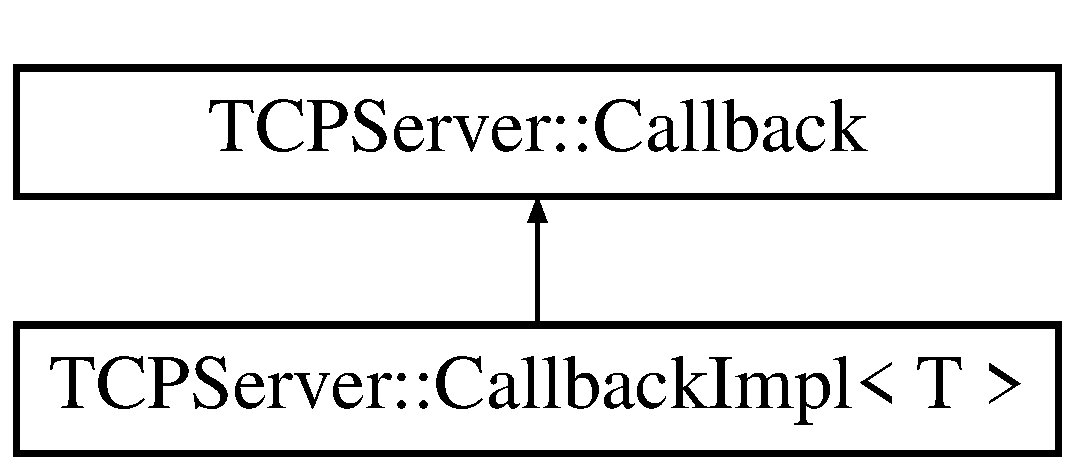
\includegraphics[height=2.000000cm]{class_t_c_p_server_1_1_callback_impl}
\end{center}
\end{figure}
\subsection*{Public Member Functions}
\begin{DoxyCompactItemize}
\item 
\hypertarget{class_t_c_p_server_1_1_callback_impl_a39abe4ac0e2782d2ec0504a01fcdeb1e}{{\bfseries Callback\-Impl} (T $\ast$obj, Func func)}\label{class_t_c_p_server_1_1_callback_impl_a39abe4ac0e2782d2ec0504a01fcdeb1e}

\item 
\hypertarget{class_t_c_p_server_1_1_callback_impl_a7370ad2f2dc50df8f623480f1991381b}{virtual bool {\bfseries call\-Func} (\hyperlink{class_t_c_p_server_1_1_cnx}{Cnx} \&cnx, const std\-::string \&request, std\-::string \&response)}\label{class_t_c_p_server_1_1_callback_impl_a7370ad2f2dc50df8f623480f1991381b}

\end{DoxyCompactItemize}


The documentation for this class was generated from the following file\-:\begin{DoxyCompactItemize}
\item 
T\-C\-P\-Server.\-h\end{DoxyCompactItemize}

\hypertarget{class_t_c_p_server_1_1_cnx}{\section{T\-C\-P\-Server\-:\-:Cnx Class Reference}
\label{class_t_c_p_server_1_1_cnx}\index{T\-C\-P\-Server\-::\-Cnx@{T\-C\-P\-Server\-::\-Cnx}}
}


represents a connection with a given client.  




{\ttfamily \#include $<$T\-C\-P\-Server.\-h$>$}

Inheritance diagram for T\-C\-P\-Server\-:\-:Cnx\-:\begin{figure}[H]
\begin{center}
\leavevmode
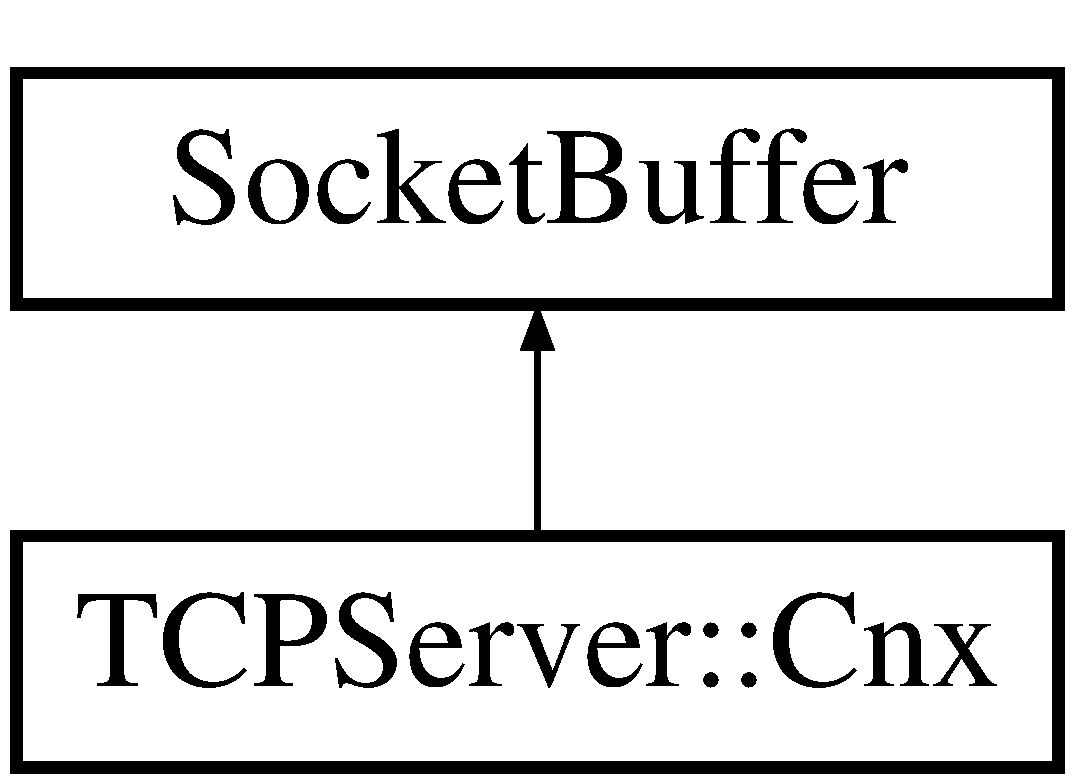
\includegraphics[height=2.000000cm]{class_t_c_p_server_1_1_cnx}
\end{center}
\end{figure}
\subsection*{Public Member Functions}
\begin{DoxyCompactItemize}
\item 
\hypertarget{class_t_c_p_server_1_1_cnx_affe5198f5dca75da9f651e286a289b47}{\hyperlink{class_t_c_p_server}{T\-C\-P\-Server} $\ast$ {\bfseries server} ()}\label{class_t_c_p_server_1_1_cnx_affe5198f5dca75da9f651e286a289b47}

\item 
\hypertarget{class_t_c_p_server_1_1_cnx_a3dd1fff38f6463d62ef5f3cae4fad340}{pthread\-\_\-t {\bfseries thread} ()}\label{class_t_c_p_server_1_1_cnx_a3dd1fff38f6463d62ef5f3cae4fad340}

\end{DoxyCompactItemize}
\subsection*{Friends}
\begin{DoxyCompactItemize}
\item 
\hypertarget{class_t_c_p_server_1_1_cnx_ae4cfdb1814d91a8d28dadb49adda68f0}{class {\bfseries T\-C\-P\-Server}}\label{class_t_c_p_server_1_1_cnx_ae4cfdb1814d91a8d28dadb49adda68f0}

\end{DoxyCompactItemize}
\subsection*{Additional Inherited Members}


\subsection{Detailed Description}
represents a connection with a given client. 

The documentation for this class was generated from the following files\-:\begin{DoxyCompactItemize}
\item 
T\-C\-P\-Server.\-h\item 
T\-C\-P\-Server.\-cpp\end{DoxyCompactItemize}

\hypertarget{class_factory}{\section{Factory Class Reference}
\label{class_factory}\index{Factory@{Factory}}
}
\subsection*{Public Member Functions}
\begin{DoxyCompactItemize}
\item 
\hypertarget{class_factory_ae6742d502be528d8ed9372dc1971f872}{std\-::shared\-\_\-ptr$<$ \hyperlink{class_multimedia}{Multimedia} $>$ {\bfseries create\-Film} (const std\-::string \&path, const std\-::string \&name)}\label{class_factory_ae6742d502be528d8ed9372dc1971f872}

\item 
\hypertarget{class_factory_ad5e2fe94c0d667d895b91f15f66910d2}{std\-::shared\-\_\-ptr$<$ \hyperlink{class_multimedia}{Multimedia} $>$ {\bfseries create\-Video} (const std\-::string \&path, const std\-::string \&name)}\label{class_factory_ad5e2fe94c0d667d895b91f15f66910d2}

\item 
\hypertarget{class_factory_a6f422e72bec7bcdaac528b1a14609ff5}{std\-::shared\-\_\-ptr$<$ \hyperlink{class_multimedia}{Multimedia} $>$ {\bfseries create\-Photo} (const std\-::string \&path, const std\-::string \&name)}\label{class_factory_a6f422e72bec7bcdaac528b1a14609ff5}

\item 
\hypertarget{class_factory_ae44fed6cd7f54edbded7d01f3a761d73}{std\-::shared\-\_\-ptr$<$ \hyperlink{class_multimedia}{Multimedia} $>$ {\bfseries create\-Group} (const std\-::string \&name)}\label{class_factory_ae44fed6cd7f54edbded7d01f3a761d73}

\item 
\hypertarget{class_factory_aa94aa2b2e3127c5298209f201c4e356f}{std\-::shared\-\_\-ptr$<$ \hyperlink{class_multimedia}{Multimedia} $>$ {\bfseries create\-Group} (const std\-::string \&name, const std\-::list$<$ std\-::shared\-\_\-ptr$<$ \hyperlink{class_multimedia}{Multimedia} $>$ $>$ \&l)}\label{class_factory_aa94aa2b2e3127c5298209f201c4e356f}

\item 
\hypertarget{class_factory_a55d75bb11685bd4f921fe8a014b3f0a5}{void \hyperlink{class_factory_a55d75bb11685bd4f921fe8a014b3f0a5}{add\-Multimedia} (const std\-::string \&name, std\-::shared\-\_\-ptr$<$ \hyperlink{class_multimedia}{Multimedia} $>$ multimedia)}\label{class_factory_a55d75bb11685bd4f921fe8a014b3f0a5}

\begin{DoxyCompactList}\small\item\em Add multimedia object (can be a group) inside the name referenced map of multimedia objects. \end{DoxyCompactList}\item 
\hypertarget{class_factory_a21b79ba789374d4ab5c44dcfb4c1542f}{void \hyperlink{class_factory_a21b79ba789374d4ab5c44dcfb4c1542f}{add\-Multimedia\-Group} (const std\-::string \&name, std\-::shared\-\_\-ptr$<$ \hyperlink{class_group}{Group}$<$ \hyperlink{class_multimedia}{Multimedia} $>$ $>$ multimedia)}\label{class_factory_a21b79ba789374d4ab5c44dcfb4c1542f}

\begin{DoxyCompactList}\small\item\em Add group of multimedia object inside the name referenced map of group objects. \end{DoxyCompactList}\item 
\hypertarget{class_factory_ad0553a33a3e6bd24614b0d645f7906e4}{bool \hyperlink{class_factory_ad0553a33a3e6bd24614b0d645f7906e4}{delete\-By\-Name} (const std\-::string \&name)}\label{class_factory_ad0553a33a3e6bd24614b0d645f7906e4}

\begin{DoxyCompactList}\small\item\em Delete an object by its name, either if it's in map of multimedia objects or in map of group objects. Return true if some objects have been found and deleted. \end{DoxyCompactList}\item 
\hypertarget{class_factory_a1e9f22828141fcb6e4f06ba8d93325f7}{std\-::shared\-\_\-ptr$<$ \hyperlink{class_multimedia}{Multimedia} $>$ \hyperlink{class_factory_a1e9f22828141fcb6e4f06ba8d93325f7}{search\-By\-Name} (const std\-::string \&name)}\label{class_factory_a1e9f22828141fcb6e4f06ba8d93325f7}

\begin{DoxyCompactList}\small\item\em Search an object by its name, only if it's in map of multimedia objects. \end{DoxyCompactList}\item 
\hypertarget{class_factory_a4c9ab55f5a833bfcb687405181936df7}{void \hyperlink{class_factory_a4c9ab55f5a833bfcb687405181936df7}{print\-By\-Name} (const std\-::string \&name)}\label{class_factory_a4c9ab55f5a833bfcb687405181936df7}

\begin{DoxyCompactList}\small\item\em Print an object by its name, either if it's in map of multimedia objects or in map of group objects. \end{DoxyCompactList}\item 
\hypertarget{class_factory_a3be1c89ec4c2b21f3fc9b0913228ee01}{void \hyperlink{class_factory_a3be1c89ec4c2b21f3fc9b0913228ee01}{print\-By\-Name} (const std\-::string \&name, std\-::ostream \&stream)}\label{class_factory_a3be1c89ec4c2b21f3fc9b0913228ee01}

\begin{DoxyCompactList}\small\item\em Print an object by its name in argument ostream, either if it's in map of multimedia objects or in map of group objects. \end{DoxyCompactList}\item 
\hypertarget{class_factory_ae08ccdd647ca3503d389f97dad8ad72d}{void \hyperlink{class_factory_ae08ccdd647ca3503d389f97dad8ad72d}{play} (const std\-::string \&name)}\label{class_factory_ae08ccdd647ca3503d389f97dad8ad72d}

\begin{DoxyCompactList}\small\item\em Call the execute method an object identified by its name, either if it's in map of multimedia objects or in map of group objects. \end{DoxyCompactList}\item 
\hypertarget{class_factory_ad520fe27ab831b5a1879ac5944ac457f}{std\-::ostream \& {\bfseries operator$<$$<$} (std\-::ostream \&oss) const }\label{class_factory_ad520fe27ab831b5a1879ac5944ac457f}

\item 
\hypertarget{class_factory_a2dc9d7912b475d5a1ff1a7655c762e5f}{std\-::ostream \& {\bfseries print} (std\-::ostream \&oss) const }\label{class_factory_a2dc9d7912b475d5a1ff1a7655c762e5f}

\item 
\hypertarget{class_factory_a6a83203ab543cb798a82bd95f774c9a3}{void \hyperlink{class_factory_a6a83203ab543cb798a82bd95f774c9a3}{throw\-If\-Bad\-Name} (const std\-::string \&name)}\label{class_factory_a6a83203ab543cb798a82bd95f774c9a3}

\begin{DoxyCompactList}\small\item\em Create exception in case of bad name (ascii$<$32 or ascii$>$127 for at least 1 char in the name) \end{DoxyCompactList}\item 
\hypertarget{class_factory_a83303191fff07dbf7f8ce4d532b2d901}{void \hyperlink{class_factory_a83303191fff07dbf7f8ce4d532b2d901}{throw\-If\-Name\-Exists\-In\-Multimedia} (const std\-::string \&name)}\label{class_factory_a83303191fff07dbf7f8ce4d532b2d901}

\begin{DoxyCompactList}\small\item\em Create exception in case of existing multimedia object. \end{DoxyCompactList}\item 
\hypertarget{class_factory_abdeccb8a1d76a56892347b01210a3388}{void \hyperlink{class_factory_abdeccb8a1d76a56892347b01210a3388}{throw\-If\-Name\-Exists\-In\-Groups} (const std\-::string \&name)}\label{class_factory_abdeccb8a1d76a56892347b01210a3388}

\begin{DoxyCompactList}\small\item\em Create exception in case of existing group object. \end{DoxyCompactList}\end{DoxyCompactItemize}


The documentation for this class was generated from the following files\-:\begin{DoxyCompactItemize}
\item 
Factory.\-hpp\item 
Factory.\-cpp\end{DoxyCompactItemize}

\hypertarget{class_film}{\section{Film Class Reference}
\label{class_film}\index{Film@{Film}}
}
Inheritance diagram for Film\-:\begin{figure}[H]
\begin{center}
\leavevmode
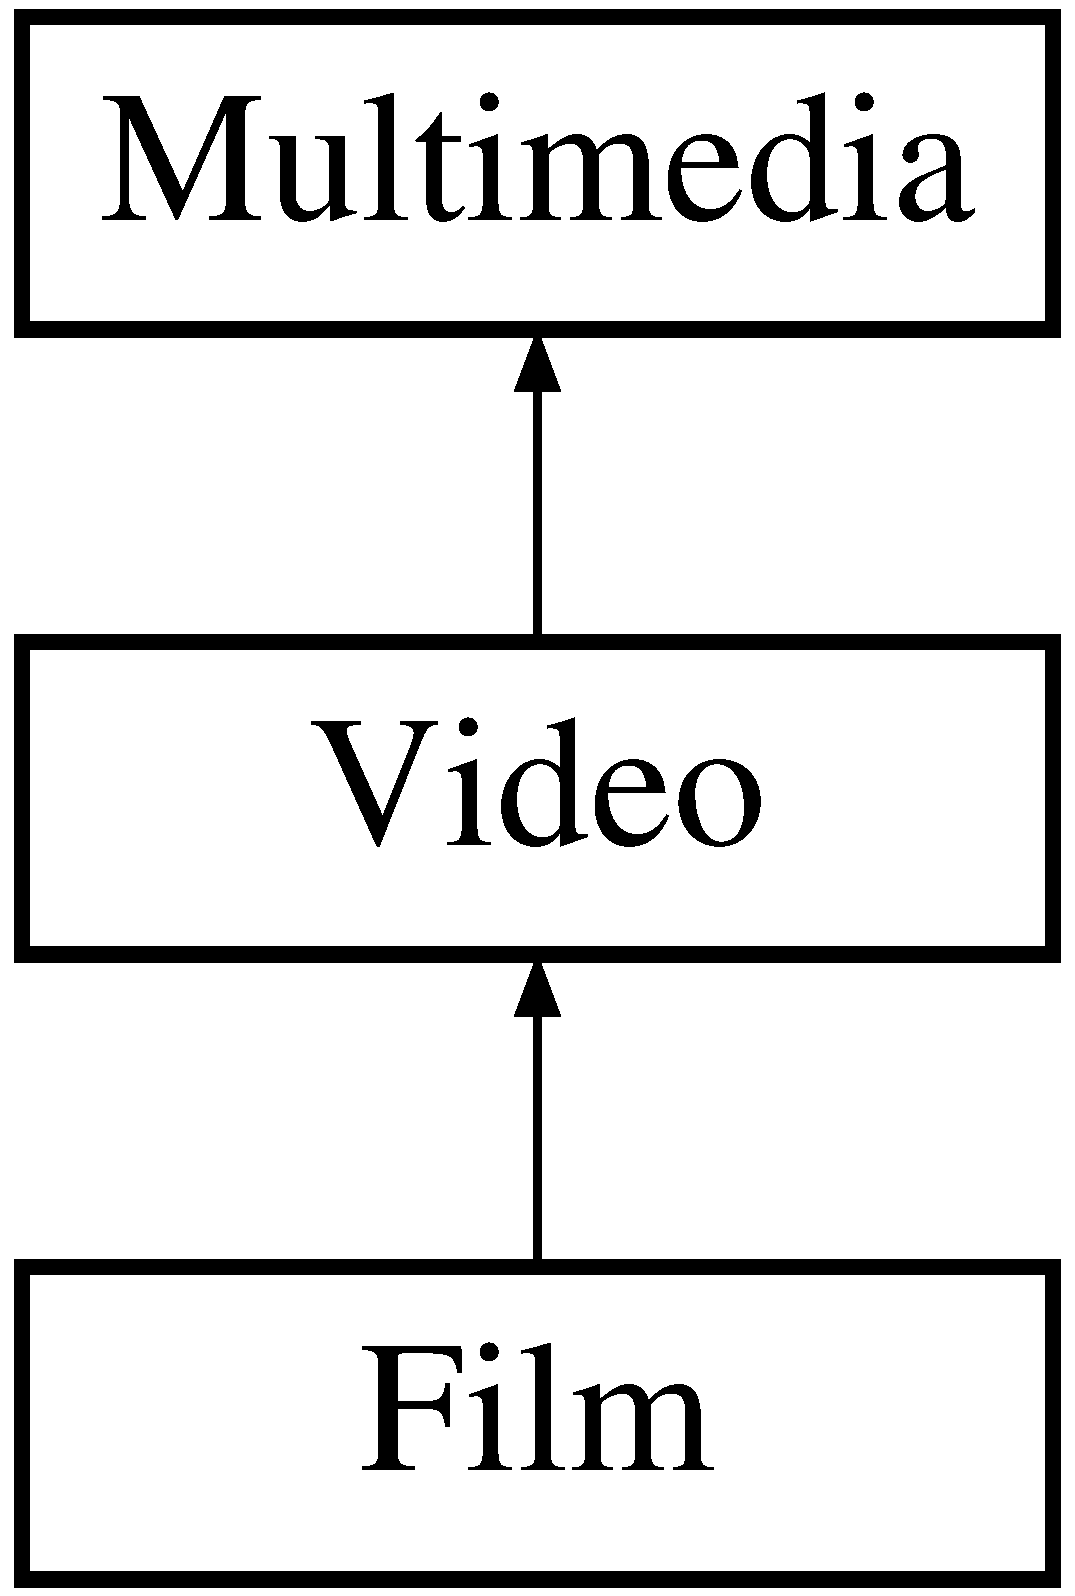
\includegraphics[height=3.000000cm]{class_film}
\end{center}
\end{figure}
\subsection*{Public Member Functions}
\begin{DoxyCompactItemize}
\item 
\hypertarget{class_film_a7a13b286528330495b2b7bc5b2a2214c}{{\bfseries Film} (int delay)}\label{class_film_a7a13b286528330495b2b7bc5b2a2214c}

\item 
\hypertarget{class_film_a3fad6e511f2e1933d8a3a7507c55aba9}{{\bfseries Film} (const std\-::string \&name, const std\-::string \&path, int delay=0)}\label{class_film_a3fad6e511f2e1933d8a3a7507c55aba9}

\item 
\hypertarget{class_film_ab364efe0650fb42f68373976e6cdae8d}{{\bfseries Film} (const std\-::string \&name, const std\-::string \&path, int $\ast$chapters, unsigned int chapter\-Number)}\label{class_film_ab364efe0650fb42f68373976e6cdae8d}

\item 
\hypertarget{class_film_a55720d8df910ce4094dde2625a091c82}{{\bfseries Film} (const \hyperlink{class_film}{Film} \&film)}\label{class_film_a55720d8df910ce4094dde2625a091c82}

\item 
\hypertarget{class_film_aa0c06810ba54f8ad9cf458dc8a0f4e19}{\hyperlink{class_film}{Film} \& \hyperlink{class_film_aa0c06810ba54f8ad9cf458dc8a0f4e19}{operator=} (const \hyperlink{class_film}{Film} \&film)}\label{class_film_aa0c06810ba54f8ad9cf458dc8a0f4e19}

\begin{DoxyCompactList}\small\item\em Redefinition of affectation operator because of pointers to copy. \end{DoxyCompactList}\item 
\hypertarget{class_film_ab1bee96f2a09e9bc0dfa548ea71f035d}{std\-::ostream \& \hyperlink{class_film_ab1bee96f2a09e9bc0dfa548ea71f035d}{print} (std\-::ostream \&oss) const }\label{class_film_ab1bee96f2a09e9bc0dfa548ea71f035d}

\begin{DoxyCompactList}\small\item\em Redefinition of print method allowing child redefinition too. \end{DoxyCompactList}\item 
\hypertarget{class_film_a9c7dee0ed9415d83ef9fe95f59961c80}{void {\bfseries set\-Chapters\-Relative} (int $\ast$chapters, unsigned int chapter\-Number)}\label{class_film_a9c7dee0ed9415d83ef9fe95f59961c80}

\item 
\hypertarget{class_film_a08bd138cdeddb5a78525e08d5d18b860}{void {\bfseries set\-Chapters} (int $\ast$chapters, unsigned int chapter\-Number)}\label{class_film_a08bd138cdeddb5a78525e08d5d18b860}

\item 
\hypertarget{class_film_a0a065380396364f453d9aa12c81587d6}{const int $\ast$const {\bfseries get\-Chapters} () const }\label{class_film_a0a065380396364f453d9aa12c81587d6}

\item 
\hypertarget{class_film_a8330191ab410d94e59e0a367f5e7c39d}{unsigned int {\bfseries get\-Chapter\-Number} () const }\label{class_film_a8330191ab410d94e59e0a367f5e7c39d}

\end{DoxyCompactItemize}
\subsection*{Additional Inherited Members}


The documentation for this class was generated from the following files\-:\begin{DoxyCompactItemize}
\item 
Film.\-hpp\item 
Film.\-cpp\end{DoxyCompactItemize}

\hypertarget{class_group}{\section{Group$<$ T $>$ Class Template Reference}
\label{class_group}\index{Group$<$ T $>$@{Group$<$ T $>$}}
}
Inheritance diagram for Group$<$ T $>$\-:\begin{figure}[H]
\begin{center}
\leavevmode
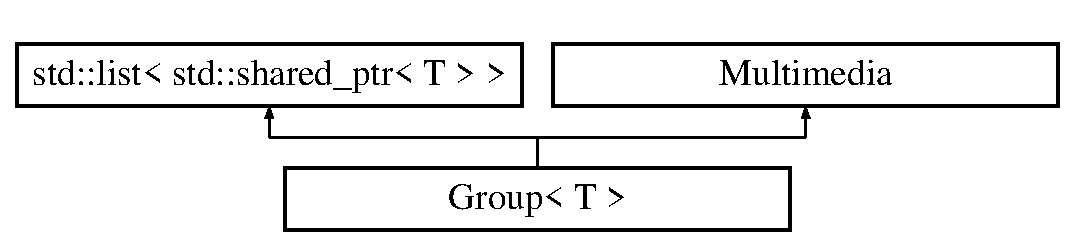
\includegraphics[height=2.000000cm]{class_group}
\end{center}
\end{figure}
\subsection*{Public Member Functions}
\begin{DoxyCompactItemize}
\item 
\hypertarget{class_group_af5e1e4f88f2ef4c53eaaf8833f1d4c56}{{\bfseries Group} (const std\-::string \&name)}\label{class_group_af5e1e4f88f2ef4c53eaaf8833f1d4c56}

\item 
\hypertarget{class_group_ac82298c5f46348f6ad7ed544e886e859}{{\bfseries Group} (const std\-::string \&name, const std\-::list$<$ std\-::shared\-\_\-ptr$<$ T $>$ $>$ \&l)}\label{class_group_ac82298c5f46348f6ad7ed544e886e859}

\item 
\hypertarget{class_group_a0554f19ad7a9e944050db55b8d051a8f}{std\-::ostream \& \hyperlink{class_group_a0554f19ad7a9e944050db55b8d051a8f}{print} (std\-::ostream \&oss) const }\label{class_group_a0554f19ad7a9e944050db55b8d051a8f}

\begin{DoxyCompactList}\small\item\em Redefinition of print method. \end{DoxyCompactList}\item 
\hypertarget{class_group_a978a041512fc9aaf91a80621a64c1d4c}{void \hyperlink{class_group_a978a041512fc9aaf91a80621a64c1d4c}{execute} () const }\label{class_group_a978a041512fc9aaf91a80621a64c1d4c}

\begin{DoxyCompactList}\small\item\em Redefinition of execute method \-: that executes all the execute methods of objects in group. \end{DoxyCompactList}\item 
\hypertarget{class_group_a91f595359a983e41f4abb2b6fbc393ce}{void {\bfseries set\-Name} (const std\-::string \&str)}\label{class_group_a91f595359a983e41f4abb2b6fbc393ce}

\item 
\hypertarget{class_group_afea29527a3a2f1c6ac7d342cce752074}{std\-::string {\bfseries get\-Name} () const }\label{class_group_afea29527a3a2f1c6ac7d342cce752074}

\end{DoxyCompactItemize}
\subsection*{Additional Inherited Members}


The documentation for this class was generated from the following file\-:\begin{DoxyCompactItemize}
\item 
Group.\-hpp\end{DoxyCompactItemize}

\hypertarget{struct_input_buffer}{\section{Input\-Buffer Struct Reference}
\label{struct_input_buffer}\index{Input\-Buffer@{Input\-Buffer}}
}
\subsection*{Public Member Functions}
\begin{DoxyCompactItemize}
\item 
\hypertarget{struct_input_buffer_a9409ec8e4581caa99dcac1af963349b5}{{\bfseries Input\-Buffer} (size\-\_\-t size)}\label{struct_input_buffer_a9409ec8e4581caa99dcac1af963349b5}

\end{DoxyCompactItemize}
\subsection*{Public Attributes}
\begin{DoxyCompactItemize}
\item 
\hypertarget{struct_input_buffer_aee7a717b6cf023deabe9910410e6cfb6}{char $\ast$ {\bfseries buffer}}\label{struct_input_buffer_aee7a717b6cf023deabe9910410e6cfb6}

\item 
\hypertarget{struct_input_buffer_a2f05121c4fb8571845cc22d083c6da46}{char $\ast$ {\bfseries begin}}\label{struct_input_buffer_a2f05121c4fb8571845cc22d083c6da46}

\item 
\hypertarget{struct_input_buffer_a52ba71c71b9b955b8369fc5217e3c4b6}{char $\ast$ {\bfseries end}}\label{struct_input_buffer_a52ba71c71b9b955b8369fc5217e3c4b6}

\item 
\hypertarget{struct_input_buffer_a621d633184a77c449e7b07d705870ae2}{ssize\-\_\-t {\bfseries remaining}}\label{struct_input_buffer_a621d633184a77c449e7b07d705870ae2}

\end{DoxyCompactItemize}


The documentation for this struct was generated from the following file\-:\begin{DoxyCompactItemize}
\item 
Socket.\-cpp\end{DoxyCompactItemize}

\hypertarget{class_t_c_p_server_1_1_lock}{\section{T\-C\-P\-Server\-:\-:Lock Class Reference}
\label{class_t_c_p_server_1_1_lock}\index{T\-C\-P\-Server\-::\-Lock@{T\-C\-P\-Server\-::\-Lock}}
}


locks the server in read mode or in write mode. In order to avoid concurrency problems between threads, the callback method that processes requests should instantiate a \hyperlink{class_t_c_p_server_1_1_lock}{Lock} object in the stack. The \hyperlink{class_t_c_p_server_1_1_lock}{Lock} must be instantiated in write mode if the request changes data, or in read mode otherwise. A write lock blocks all other locks (hence, all other threads) until the callback method that issued the write lock returns.  




{\ttfamily \#include $<$T\-C\-P\-Server.\-h$>$}

\subsection*{Public Member Functions}
\begin{DoxyCompactItemize}
\item 
\hypertarget{class_t_c_p_server_1_1_lock_a4b1fa591dde407aacd93133828cfac81}{\hyperlink{class_t_c_p_server_1_1_lock_a4b1fa591dde407aacd93133828cfac81}{Lock} (\hyperlink{class_t_c_p_server_1_1_cnx}{Cnx} \&, bool write\-Mode=false)}\label{class_t_c_p_server_1_1_lock_a4b1fa591dde407aacd93133828cfac81}

\begin{DoxyCompactList}\small\item\em locks the connection in write mode if the second argument is true and in read mode otherwise. \end{DoxyCompactList}\end{DoxyCompactItemize}


\subsection{Detailed Description}
locks the server in read mode or in write mode. In order to avoid concurrency problems between threads, the callback method that processes requests should instantiate a \hyperlink{class_t_c_p_server_1_1_lock}{Lock} object in the stack. The \hyperlink{class_t_c_p_server_1_1_lock}{Lock} must be instantiated in write mode if the request changes data, or in read mode otherwise. A write lock blocks all other locks (hence, all other threads) until the callback method that issued the write lock returns. 

The documentation for this class was generated from the following files\-:\begin{DoxyCompactItemize}
\item 
T\-C\-P\-Server.\-h\item 
T\-C\-P\-Server.\-cpp\end{DoxyCompactItemize}

\hypertarget{class_multimedia}{\section{Multimedia Class Reference}
\label{class_multimedia}\index{Multimedia@{Multimedia}}
}
Inheritance diagram for Multimedia\-:\begin{figure}[H]
\begin{center}
\leavevmode
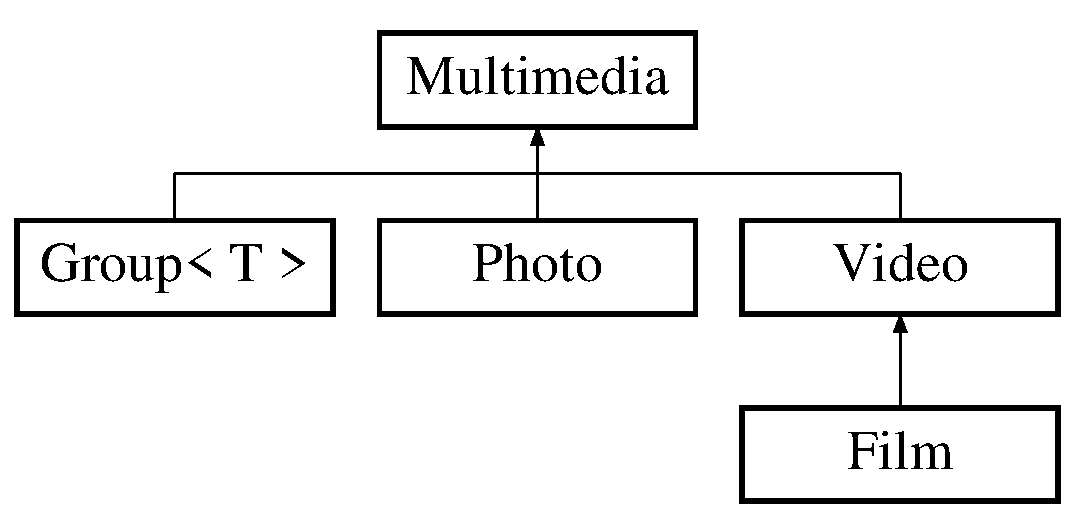
\includegraphics[height=3.000000cm]{class_multimedia}
\end{center}
\end{figure}
\subsection*{Public Member Functions}
\begin{DoxyCompactItemize}
\item 
\hypertarget{class_multimedia_ac51930f687bcb9fd44392932c1f0e631}{{\bfseries Multimedia} (const std\-::string \&name=\char`\"{}\char`\"{}, const std\-::string \&path=\char`\"{}\char`\"{})}\label{class_multimedia_ac51930f687bcb9fd44392932c1f0e631}

\item 
\hypertarget{class_multimedia_aa4be8fe3f1749c95bc2bf591dd836b56}{std\-::ostream \& \hyperlink{class_multimedia_aa4be8fe3f1749c95bc2bf591dd836b56}{operator$<$$<$} (std\-::ostream \&oss) const }\label{class_multimedia_aa4be8fe3f1749c95bc2bf591dd836b56}

\begin{DoxyCompactList}\small\item\em Redefinition of operator $<$$<$ in order to print objects easily. \end{DoxyCompactList}\item 
virtual std\-::ostream \& \hyperlink{class_multimedia_a90d8b3e78733443b358409b117c14ffd}{print} (std\-::ostream \&oss) const 
\begin{DoxyCompactList}\small\item\em The virtual method print allow a redefinition of the way we want to print certain objects. \end{DoxyCompactList}\item 
\hypertarget{class_multimedia_adcabfa7365b1974a7911ae025815ec39}{virtual void \hyperlink{class_multimedia_adcabfa7365b1974a7911ae025815ec39}{execute} () const }\label{class_multimedia_adcabfa7365b1974a7911ae025815ec39}

\begin{DoxyCompactList}\small\item\em The virtual method execute allow playing the resource on the server. \end{DoxyCompactList}\item 
\hypertarget{class_multimedia_a7f76261a215bae20b9fafa18acb5ebd2}{void {\bfseries set\-Name} (const std\-::string \&name)}\label{class_multimedia_a7f76261a215bae20b9fafa18acb5ebd2}

\item 
\hypertarget{class_multimedia_a79367ce0f6fbd1d0c00ddb2bd6336ebb}{void {\bfseries set\-Path} (const std\-::string \&path)}\label{class_multimedia_a79367ce0f6fbd1d0c00ddb2bd6336ebb}

\item 
\hypertarget{class_multimedia_a6fff227dbb724674af160d1bde39815d}{const std\-::string \& {\bfseries get\-Name} () const }\label{class_multimedia_a6fff227dbb724674af160d1bde39815d}

\item 
\hypertarget{class_multimedia_aa89052d06db704f571e3c1b48bddeaa6}{const std\-::string \& {\bfseries get\-Path} () const }\label{class_multimedia_aa89052d06db704f571e3c1b48bddeaa6}

\end{DoxyCompactItemize}
\subsection*{Protected Attributes}
\begin{DoxyCompactItemize}
\item 
\hypertarget{class_multimedia_a58f835cc9f6520566094574971ce4033}{std\-::string {\bfseries name}}\label{class_multimedia_a58f835cc9f6520566094574971ce4033}

\item 
\hypertarget{class_multimedia_a63d0bda0f1905b61fb18f53f3384644d}{std\-::string {\bfseries path}}\label{class_multimedia_a63d0bda0f1905b61fb18f53f3384644d}

\end{DoxyCompactItemize}


\subsection{Member Function Documentation}
\hypertarget{class_multimedia_a90d8b3e78733443b358409b117c14ffd}{\index{Multimedia@{Multimedia}!print@{print}}
\index{print@{print}!Multimedia@{Multimedia}}
\subsubsection[{print}]{\setlength{\rightskip}{0pt plus 5cm}std\-::ostream \& Multimedia\-::print (
\begin{DoxyParamCaption}
\item[{std\-::ostream \&}]{oss}
\end{DoxyParamCaption}
) const\hspace{0.3cm}{\ttfamily [virtual]}}}\label{class_multimedia_a90d8b3e78733443b358409b117c14ffd}


The virtual method print allow a redefinition of the way we want to print certain objects. 

Default print method. 

Reimplemented in \hyperlink{class_film_ab1bee96f2a09e9bc0dfa548ea71f035d}{Film}, \hyperlink{class_group_a0554f19ad7a9e944050db55b8d051a8f}{Group$<$ T $>$}, \hyperlink{class_photo_aad7279a92e29492342ce2708b3d7e417}{Photo}, and \hyperlink{class_video_a1bd10186658fb7399508bd43c3dc6c51}{Video}.



The documentation for this class was generated from the following files\-:\begin{DoxyCompactItemize}
\item 
Multimedia.\-hpp\item 
Multimedia.\-cpp\end{DoxyCompactItemize}

\hypertarget{class_photo}{\section{Photo Class Reference}
\label{class_photo}\index{Photo@{Photo}}
}
Inheritance diagram for Photo\-:\begin{figure}[H]
\begin{center}
\leavevmode
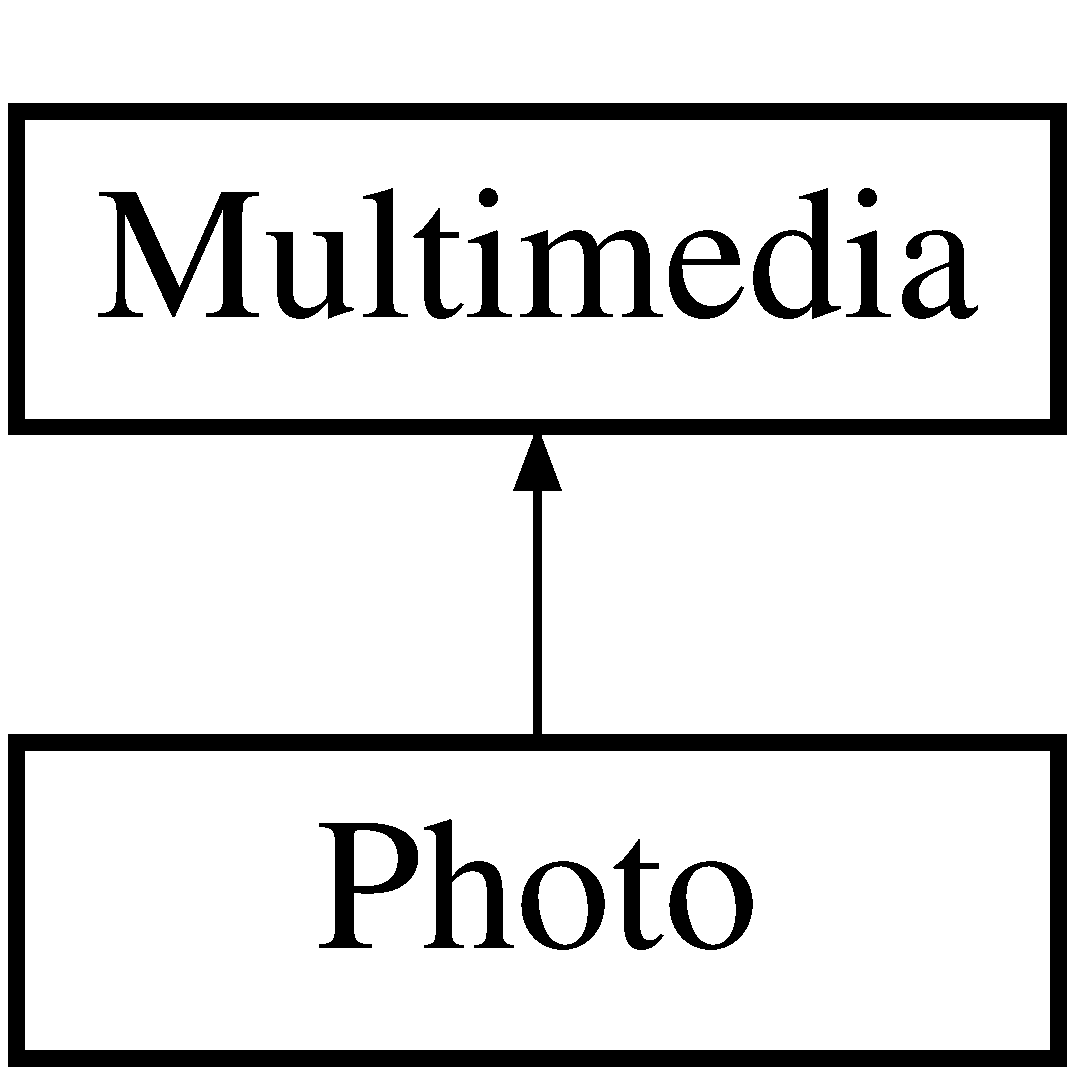
\includegraphics[height=2.000000cm]{class_photo}
\end{center}
\end{figure}
\subsection*{Public Member Functions}
\begin{DoxyCompactItemize}
\item 
\hypertarget{class_photo_a839aaf99fe6a121bed99f8e0c797557b}{{\bfseries Photo} (float lattitude, float longitude)}\label{class_photo_a839aaf99fe6a121bed99f8e0c797557b}

\item 
\hypertarget{class_photo_aa3e3af9f5042f50accabb536908a1226}{{\bfseries Photo} (const std\-::string \&name, const std\-::string \&path, float lattitude=0, float longitude=0)}\label{class_photo_aa3e3af9f5042f50accabb536908a1226}

\item 
\hypertarget{class_photo_aad7279a92e29492342ce2708b3d7e417}{std\-::ostream \& \hyperlink{class_photo_aad7279a92e29492342ce2708b3d7e417}{print} (std\-::ostream \&oss) const }\label{class_photo_aad7279a92e29492342ce2708b3d7e417}

\begin{DoxyCompactList}\small\item\em Redefinition of print method. \end{DoxyCompactList}\item 
\hypertarget{class_photo_a9d4920cbf6fc466630e3a8b4d5df84db}{void \hyperlink{class_photo_a9d4920cbf6fc466630e3a8b4d5df84db}{execute} () const }\label{class_photo_a9d4920cbf6fc466630e3a8b4d5df84db}

\begin{DoxyCompactList}\small\item\em Open the photo inside Unix environment (doesn't work within windows if no unix environment with display command is installed) \end{DoxyCompactList}\item 
\hypertarget{class_photo_a2e7159e2ebbd5ca993ae746825e4700b}{void {\bfseries set\-Lattitude} (float lattitude)}\label{class_photo_a2e7159e2ebbd5ca993ae746825e4700b}

\item 
\hypertarget{class_photo_a9214ffc09168ae3a8134381c22266f91}{void {\bfseries set\-Longitude} (float lattitude)}\label{class_photo_a9214ffc09168ae3a8134381c22266f91}

\item 
\hypertarget{class_photo_ab02d0f97243f927d0fbf311712a96118}{float {\bfseries get\-Lattitude} () const }\label{class_photo_ab02d0f97243f927d0fbf311712a96118}

\item 
\hypertarget{class_photo_a02787b27b9d7c919e9ecfaa2e99a1862}{float {\bfseries get\-Longitude} () const }\label{class_photo_a02787b27b9d7c919e9ecfaa2e99a1862}

\end{DoxyCompactItemize}
\subsection*{Additional Inherited Members}


The documentation for this class was generated from the following files\-:\begin{DoxyCompactItemize}
\item 
Photo.\-hpp\item 
Photo.\-cpp\end{DoxyCompactItemize}

\hypertarget{class_process_request}{\section{Process\-Request Class Reference}
\label{class_process_request}\index{Process\-Request@{Process\-Request}}
}
\subsection*{Public Member Functions}
\begin{DoxyCompactItemize}
\item 
\hypertarget{class_process_request_a4b873e251b1d64c66e13864c64523305}{{\bfseries Process\-Request} (const std\-::shared\-\_\-ptr$<$ \hyperlink{class_factory}{Factory} $>$ \&factory)}\label{class_process_request_a4b873e251b1d64c66e13864c64523305}

\item 
\hypertarget{class_process_request_ae47375579973072ebddfc554b991d80b}{bool \hyperlink{class_process_request_ae47375579973072ebddfc554b991d80b}{process} (\hyperlink{class_t_c_p_server_1_1_cnx}{T\-C\-P\-Server\-::\-Cnx} \&cnx, const std\-::string \&request, std\-::string \&response)}\label{class_process_request_ae47375579973072ebddfc554b991d80b}

\begin{DoxyCompactList}\small\item\em Process the request which comes from network. \end{DoxyCompactList}\end{DoxyCompactItemize}


The documentation for this class was generated from the following files\-:\begin{DoxyCompactItemize}
\item 
Processrequest.\-hpp\item 
Processrequest.\-cpp\end{DoxyCompactItemize}

\hypertarget{class_server_socket}{\section{Server\-Socket Class Reference}
\label{class_server_socket}\index{Server\-Socket@{Server\-Socket}}
}


T\-C\-P/\-I\-P \hyperlink{class_socket}{Socket} Server. This class encapsulates a T\-C\-P/\-I\-P socket server. A\-F\-\_\-\-I\-N\-E\-T connections following the I\-Pv4 Internet protocol are supported.  




{\ttfamily \#include $<$Socket.\-h$>$}

\subsection*{Public Member Functions}
\begin{DoxyCompactItemize}
\item 
\hypertarget{class_server_socket_a2b3098589541243241ca25495155186c}{\hyperlink{class_server_socket_a2b3098589541243241ca25495155186c}{Server\-Socket} ()}\label{class_server_socket_a2b3098589541243241ca25495155186c}

\begin{DoxyCompactList}\small\item\em Creates a new server socket. Creates a listening socket that waits for connection requests by T\-C\-P/\-I\-P clients. \end{DoxyCompactList}\item 
virtual \hyperlink{class_socket}{Socket} $\ast$ \hyperlink{class_server_socket_accc3d56d42aa50a5f3c920cf0b26959b}{accept} ()
\begin{DoxyCompactList}\small\item\em Accepts a new connection request and returns the corresponding socket. By default, this function blocks the caller until a connection is present. \end{DoxyCompactList}\item 
virtual int \hyperlink{class_server_socket_ad5281fe6c005bca007a9a758bd612481}{bind} (int port, int backlog=50)
\begin{DoxyCompactList}\small\item\em Assigns the socket to the local address. The socket must be bound before using it. \end{DoxyCompactList}\item 
\hypertarget{class_server_socket_a3eac6d5571bb092622d328dbda2de2cf}{virtual int \hyperlink{class_server_socket_a3eac6d5571bb092622d328dbda2de2cf}{close} ()}\label{class_server_socket_a3eac6d5571bb092622d328dbda2de2cf}

\begin{DoxyCompactList}\small\item\em Closes the socket. \end{DoxyCompactList}\item 
\hypertarget{class_server_socket_ad5b053b711f97cfe8b56f6febc15df65}{bool \hyperlink{class_server_socket_ad5b053b711f97cfe8b56f6febc15df65}{is\-Closed} () const }\label{class_server_socket_ad5b053b711f97cfe8b56f6febc15df65}

\begin{DoxyCompactList}\small\item\em Returns true if the socket has been closed. \end{DoxyCompactList}\item 
\hypertarget{class_server_socket_a57b5b84a60906153d9755190cdfd0d39}{int \hyperlink{class_server_socket_a57b5b84a60906153d9755190cdfd0d39}{descriptor} ()}\label{class_server_socket_a57b5b84a60906153d9755190cdfd0d39}

\begin{DoxyCompactList}\small\item\em Returns the Unix descriptor of the socket. \end{DoxyCompactList}\item 
\hypertarget{class_server_socket_ab34154bc6114c638ae02f5e018121099}{int \hyperlink{class_server_socket_ab34154bc6114c638ae02f5e018121099}{set\-Receive\-Buffer\-Size} (int size)}\label{class_server_socket_ab34154bc6114c638ae02f5e018121099}

\begin{DoxyCompactList}\small\item\em Sets the S\-O\-\_\-\-R\-C\-V\-B\-U\-F option to the specified value. \end{DoxyCompactList}\item 
\hypertarget{class_server_socket_ae60d7cc31ad535e5d3cac42e38b8ec98}{int \hyperlink{class_server_socket_ae60d7cc31ad535e5d3cac42e38b8ec98}{set\-Reuse\-Address} (bool)}\label{class_server_socket_ae60d7cc31ad535e5d3cac42e38b8ec98}

\begin{DoxyCompactList}\small\item\em Enables/disables the S\-O\-\_\-\-R\-E\-U\-S\-E\-A\-D\-D\-R socket option. \end{DoxyCompactList}\item 
\hypertarget{class_server_socket_aedb9144c9c375fcb14ac47bcb9d2eb17}{int \hyperlink{class_server_socket_aedb9144c9c375fcb14ac47bcb9d2eb17}{set\-So\-Timeout} (int timeout)}\label{class_server_socket_aedb9144c9c375fcb14ac47bcb9d2eb17}

\begin{DoxyCompactList}\small\item\em Enables/disables S\-O\-\_\-\-T\-I\-M\-E\-O\-U\-T with the specified timeout (in milliseconds). \end{DoxyCompactList}\item 
\hypertarget{class_server_socket_a9e5e1ee852ba26156c757a0086b780fe}{int \hyperlink{class_server_socket_a9e5e1ee852ba26156c757a0086b780fe}{set\-Tcp\-No\-Delay} (bool)}\label{class_server_socket_a9e5e1ee852ba26156c757a0086b780fe}

\begin{DoxyCompactList}\small\item\em Turns on/off T\-C\-P coalescence (useful in some cases to avoid delays). \end{DoxyCompactList}\end{DoxyCompactItemize}


\subsection{Detailed Description}
T\-C\-P/\-I\-P \hyperlink{class_socket}{Socket} Server. This class encapsulates a T\-C\-P/\-I\-P socket server. A\-F\-\_\-\-I\-N\-E\-T connections following the I\-Pv4 Internet protocol are supported. 

Class \hyperlink{class_socket}{Socket} should be used on the client side (\begin{DoxySeeAlso}{See Also}
\hyperlink{class_socket}{Socket}).
\end{DoxySeeAlso}
T\-C\-P/\-I\-P sockets do not preserve record boundaries, \begin{DoxySeeAlso}{See Also}
\hyperlink{class_socket_buffer}{Socket\-Buffer} for a solution. 
\end{DoxySeeAlso}


\subsection{Member Function Documentation}
\hypertarget{class_server_socket_accc3d56d42aa50a5f3c920cf0b26959b}{\index{Server\-Socket@{Server\-Socket}!accept@{accept}}
\index{accept@{accept}!ServerSocket@{Server\-Socket}}
\subsubsection[{accept}]{\setlength{\rightskip}{0pt plus 5cm}{\bf Socket} $\ast$ Server\-Socket\-::accept (
\begin{DoxyParamCaption}
{}
\end{DoxyParamCaption}
)\hspace{0.3cm}{\ttfamily [virtual]}}}\label{class_server_socket_accc3d56d42aa50a5f3c920cf0b26959b}


Accepts a new connection request and returns the corresponding socket. By default, this function blocks the caller until a connection is present. 

\begin{DoxyReturn}{Returns}
the new \hyperlink{class_socket}{Socket} or nullptr on error. 
\end{DoxyReturn}
\hypertarget{class_server_socket_ad5281fe6c005bca007a9a758bd612481}{\index{Server\-Socket@{Server\-Socket}!bind@{bind}}
\index{bind@{bind}!ServerSocket@{Server\-Socket}}
\subsubsection[{bind}]{\setlength{\rightskip}{0pt plus 5cm}int Server\-Socket\-::bind (
\begin{DoxyParamCaption}
\item[{int}]{port, }
\item[{int}]{backlog = {\ttfamily 50}}
\end{DoxyParamCaption}
)\hspace{0.3cm}{\ttfamily [virtual]}}}\label{class_server_socket_ad5281fe6c005bca007a9a758bd612481}


Assigns the socket to the local address. The socket must be bound before using it. 

\begin{DoxyReturn}{Returns}
0 on success or a negative value on error which is one of \hyperlink{class_socket_a9f68308228badcdd299cd83e62e36976}{Socket\-::\-Errors} 
\end{DoxyReturn}


The documentation for this class was generated from the following files\-:\begin{DoxyCompactItemize}
\item 
Socket.\-h\item 
Socket.\-cpp\end{DoxyCompactItemize}

\hypertarget{class_socket}{\section{Socket Class Reference}
\label{class_socket}\index{Socket@{Socket}}
}


T\-C\-P/\-I\-P or U\-D\-P/\-Datagram \hyperlink{class_socket}{Socket}. This class encapsulates a T\-C\-P/\-I\-P or U\-D\-P/\-Datagram socket. A\-F\-\_\-\-I\-N\-E\-T connections following the I\-Pv4 Internet protocol are supported.  




{\ttfamily \#include $<$Socket.\-h$>$}

\subsection*{Public Types}
\begin{DoxyCompactItemize}
\item 
enum \hyperlink{class_socket_a9f68308228badcdd299cd83e62e36976}{Errors} \{ {\bfseries Failed} = -\/1, 
{\bfseries Invalid\-Socket} = -\/2, 
{\bfseries Unknown\-Host} = -\/3
 \}
\begin{DoxyCompactList}\small\item\em \hyperlink{class_socket}{Socket} errors. \end{DoxyCompactList}\end{DoxyCompactItemize}
\subsection*{Public Member Functions}
\begin{DoxyCompactItemize}
\item 
\hyperlink{class_socket_acd3cb39bc957be2f34c91b9e262e1cec}{Socket} (int type=S\-O\-C\-K\-\_\-\-S\-T\-R\-E\-A\-M)
\begin{DoxyCompactList}\small\item\em Creates a new \hyperlink{class_socket}{Socket}. Creates a A\-F\-\_\-\-I\-N\-E\-T socket using the I\-Pv4 Internet protocol. Type can be\-: \end{DoxyCompactList}\item 
\hypertarget{class_socket_a14170941ba1aaa3263f3e8dd3f85e24f}{\hyperlink{class_socket_a14170941ba1aaa3263f3e8dd3f85e24f}{Socket} (int type, int sockfd)}\label{class_socket_a14170941ba1aaa3263f3e8dd3f85e24f}

\begin{DoxyCompactList}\small\item\em Creates a \hyperlink{class_socket}{Socket} object from an existing socket file descriptor. \end{DoxyCompactList}\item 
\hypertarget{class_socket_aeac4eb6379a543d38ed88977d3b6630a}{virtual \hyperlink{class_socket_aeac4eb6379a543d38ed88977d3b6630a}{$\sim$\-Socket} ()}\label{class_socket_aeac4eb6379a543d38ed88977d3b6630a}

\begin{DoxyCompactList}\small\item\em Destructor (closes the socket). \end{DoxyCompactList}\item 
virtual int \hyperlink{class_socket_aff8a77c02a44937db59c8c8a057072d9}{bind} (int port)
\begin{DoxyCompactList}\small\item\em Assigns the socket to the local address. Typically used for U\-D\-P/\-Datagram sockets,. \end{DoxyCompactList}\item 
virtual int \hyperlink{class_socket_a8f014a801fb3e61bbee00b84c06f2330}{bind} (const std\-::string \&host, int port)
\begin{DoxyCompactList}\small\item\em Assigns the socket to an address. Typically used for U\-D\-P/\-Datagram sockets,. \end{DoxyCompactList}\item 
virtual int \hyperlink{class_socket_a772419bd74c4fe4987d190506a64ff87}{connect} (const std\-::string \&host, int port)
\begin{DoxyCompactList}\small\item\em Connects the socket to an address. Typically used for T\-C\-P/\-I\-P sockets on the client side,. \end{DoxyCompactList}\item 
virtual int \hyperlink{class_socket_aef06605c6725958004116983f1a2051f}{close} ()
\begin{DoxyCompactList}\small\item\em Closes the socket. \end{DoxyCompactList}\item 
\hypertarget{class_socket_a6a086cd11aba1fd114dc18008dd0c6b4}{bool \hyperlink{class_socket_a6a086cd11aba1fd114dc18008dd0c6b4}{is\-Closed} () const }\label{class_socket_a6a086cd11aba1fd114dc18008dd0c6b4}

\begin{DoxyCompactList}\small\item\em Returns true if the socket has been closed. \end{DoxyCompactList}\item 
\hypertarget{class_socket_a92b54e2c8f3ae67af7c809dc119950cb}{int \hyperlink{class_socket_a92b54e2c8f3ae67af7c809dc119950cb}{descriptor} ()}\label{class_socket_a92b54e2c8f3ae67af7c809dc119950cb}

\begin{DoxyCompactList}\small\item\em Returns the Unix descriptor of the socket. \end{DoxyCompactList}\item 
ssize\-\_\-t \hyperlink{class_socket_a9275eacdb64056a53cf4b9cf54cd2f1a}{send} (const void $\ast$buf, size\-\_\-t len, int flags=0)
\begin{DoxyCompactList}\small\item\em Sends data to a connected socket. Sends {\itshape len} bytes to a T\-C\-P/\-I\-P socket. \end{DoxyCompactList}\item 
ssize\-\_\-t \hyperlink{class_socket_aa5e98b6f2c4e26fcf90d71c8386fc09d}{receive} (void $\ast$buf, size\-\_\-t len, int flags=0)
\begin{DoxyCompactList}\small\item\em Receives data from a connected socket. Reads at most {\itshape len} bytes from a T\-C\-P/\-I\-P socket. Normally, this function blocks the caller until data is present. \end{DoxyCompactList}\item 
ssize\-\_\-t \hyperlink{class_socket_ac75e3ac80b7e6ae1bdce58c1c4e2b56a}{send\-To} (const void $\ast$buf, size\-\_\-t len, int flags, const struct sockaddr $\ast$dest\-\_\-addr, socklen\-\_\-t addrlen)
\begin{DoxyCompactList}\small\item\em Sends data to a datagram socket. Sends {\itshape len} bytes to a datagram socket. \end{DoxyCompactList}\item 
ssize\-\_\-t \hyperlink{class_socket_a7cca10ce2a21e0648850e55a878f51b2}{receive\-From} (void $\ast$buf, size\-\_\-t len, int flags, struct sockaddr $\ast$src\-\_\-addr, socklen\-\_\-t $\ast$addrlen)
\begin{DoxyCompactList}\small\item\em Receives data from datagram socket. Reads at most {\itshape len} bytes from a datagram socket, Normally, this function blocks the caller until data is present. \end{DoxyCompactList}\item 
\hypertarget{class_socket_a417b47af24de10184192de00d9112589}{virtual void \hyperlink{class_socket_a417b47af24de10184192de00d9112589}{shutdown\-Input} ()}\label{class_socket_a417b47af24de10184192de00d9112589}

\begin{DoxyCompactList}\small\item\em Disables further receive operations. \end{DoxyCompactList}\item 
\hypertarget{class_socket_a650128aee2581e6695c6812d8afe14b5}{virtual void \hyperlink{class_socket_a650128aee2581e6695c6812d8afe14b5}{shutdown\-Output} ()}\label{class_socket_a650128aee2581e6695c6812d8afe14b5}

\begin{DoxyCompactList}\small\item\em Disables further send operations. \end{DoxyCompactList}\item 
\hypertarget{class_socket_a06ff0dd6837c9f51948df655fc2713cd}{int \hyperlink{class_socket_a06ff0dd6837c9f51948df655fc2713cd}{set\-Receive\-Buffer\-Size} (int size)}\label{class_socket_a06ff0dd6837c9f51948df655fc2713cd}

\begin{DoxyCompactList}\small\item\em Sets the size of the T\-C\-P/\-I\-P input buffer. \end{DoxyCompactList}\item 
\hypertarget{class_socket_ab02b997fa7e251d596116e95c9ccaf97}{int \hyperlink{class_socket_ab02b997fa7e251d596116e95c9ccaf97}{set\-Reuse\-Address} (bool)}\label{class_socket_ab02b997fa7e251d596116e95c9ccaf97}

\begin{DoxyCompactList}\small\item\em Enables/disables the S\-O\-\_\-\-R\-E\-U\-S\-E\-A\-D\-D\-R socket option. \end{DoxyCompactList}\item 
\hypertarget{class_socket_afc49ad6cc259a0006ca13bb22fdd7383}{int \hyperlink{class_socket_afc49ad6cc259a0006ca13bb22fdd7383}{set\-Send\-Buffer\-Size} (int size)}\label{class_socket_afc49ad6cc259a0006ca13bb22fdd7383}

\begin{DoxyCompactList}\small\item\em Sets the size of the T\-C\-P/\-I\-P output buffer. \end{DoxyCompactList}\item 
\hypertarget{class_socket_a41cc1caae51e3e83e16ce2c20689ed03}{int \hyperlink{class_socket_a41cc1caae51e3e83e16ce2c20689ed03}{set\-So\-Linger} (bool, int linger)}\label{class_socket_a41cc1caae51e3e83e16ce2c20689ed03}

\begin{DoxyCompactList}\small\item\em Enables/disables S\-O\-\_\-\-L\-I\-N\-G\-E\-R with the specified linger time in seconds. \end{DoxyCompactList}\item 
\hypertarget{class_socket_ad65a22ec40902e2c0a98c5d4ac885f99}{int \hyperlink{class_socket_ad65a22ec40902e2c0a98c5d4ac885f99}{set\-So\-Timeout} (int timeout)}\label{class_socket_ad65a22ec40902e2c0a98c5d4ac885f99}

\begin{DoxyCompactList}\small\item\em Enables/disables S\-O\-\_\-\-T\-I\-M\-E\-O\-U\-T with the specified timeout (in milliseconds). \end{DoxyCompactList}\item 
\hypertarget{class_socket_a7bc0110f3bedbb18f26b05ece01553fa}{int \hyperlink{class_socket_a7bc0110f3bedbb18f26b05ece01553fa}{set\-Tcp\-No\-Delay} (bool)}\label{class_socket_a7bc0110f3bedbb18f26b05ece01553fa}

\begin{DoxyCompactList}\small\item\em Enables/disables T\-C\-P\-\_\-\-N\-O\-D\-E\-L\-A\-Y (turns on/off T\-C\-P coalescence). \end{DoxyCompactList}\item 
\hypertarget{class_socket_ae7b8bde73ff163d3a92b6cc7dcb7e5cd}{int \hyperlink{class_socket_ae7b8bde73ff163d3a92b6cc7dcb7e5cd}{get\-Receive\-Buffer\-Size} () const }\label{class_socket_ae7b8bde73ff163d3a92b6cc7dcb7e5cd}

\begin{DoxyCompactList}\small\item\em Gets the size of the T\-C\-P/\-I\-P input buffer. \end{DoxyCompactList}\item 
\hypertarget{class_socket_aee4eabe73fc1550fadca23ad910d757c}{bool \hyperlink{class_socket_aee4eabe73fc1550fadca23ad910d757c}{get\-Reuse\-Address} () const }\label{class_socket_aee4eabe73fc1550fadca23ad910d757c}

\begin{DoxyCompactList}\small\item\em Gets S\-O\-\_\-\-R\-E\-U\-S\-E\-A\-D\-D\-R state. \end{DoxyCompactList}\item 
\hypertarget{class_socket_a7f899aac444facd294ef1dcfdd2cccb8}{int \hyperlink{class_socket_a7f899aac444facd294ef1dcfdd2cccb8}{get\-Send\-Buffer\-Size} () const }\label{class_socket_a7f899aac444facd294ef1dcfdd2cccb8}

\begin{DoxyCompactList}\small\item\em Gets the size of the T\-C\-P/\-I\-P output buffer. \end{DoxyCompactList}\item 
\hypertarget{class_socket_abd5f4f7ec400fba1fdc7fb4482daa43a}{bool \hyperlink{class_socket_abd5f4f7ec400fba1fdc7fb4482daa43a}{get\-So\-Linger} (int \&linger) const }\label{class_socket_abd5f4f7ec400fba1fdc7fb4482daa43a}

\begin{DoxyCompactList}\small\item\em Gets S\-O\-\_\-\-L\-I\-N\-G\-E\-R state and the specified linger time in seconds. \end{DoxyCompactList}\item 
\hypertarget{class_socket_a628371e91c172f1405ce39f44587ff34}{int \hyperlink{class_socket_a628371e91c172f1405ce39f44587ff34}{get\-So\-Timeout} () const }\label{class_socket_a628371e91c172f1405ce39f44587ff34}

\begin{DoxyCompactList}\small\item\em Gets S\-O\-\_\-\-T\-I\-M\-E\-O\-U\-T value. \end{DoxyCompactList}\item 
\hypertarget{class_socket_ab5fe067d4678d1d3ff906135e2cdbbb4}{bool \hyperlink{class_socket_ab5fe067d4678d1d3ff906135e2cdbbb4}{get\-Tcp\-No\-Delay} () const }\label{class_socket_ab5fe067d4678d1d3ff906135e2cdbbb4}

\begin{DoxyCompactList}\small\item\em Gets T\-C\-P\-\_\-\-N\-O\-D\-E\-L\-A\-Y state. \end{DoxyCompactList}\item 
\hypertarget{class_socket_ae098ebe2d34fac9947260f517ee8de04}{virtual int \hyperlink{class_socket_ae098ebe2d34fac9947260f517ee8de04}{set\-Local\-Address} (struct sockaddr\-\_\-in \&addr, int port)}\label{class_socket_ae098ebe2d34fac9947260f517ee8de04}

\begin{DoxyCompactList}\small\item\em Initializes a local I\-N\-E\-T4 address, returns 0 on success, -\/1 otherwise. \end{DoxyCompactList}\item 
\hypertarget{class_socket_aec683b1b0104aeae9fc2cfdbb6b70e9f}{virtual int \hyperlink{class_socket_aec683b1b0104aeae9fc2cfdbb6b70e9f}{set\-Address} (struct sockaddr\-\_\-in \&addr, const std\-::string \&host, int port)}\label{class_socket_aec683b1b0104aeae9fc2cfdbb6b70e9f}

\begin{DoxyCompactList}\small\item\em Initializes a remote I\-N\-E\-T4 address, returns 0 on success, -\/1 otherwise. \end{DoxyCompactList}\end{DoxyCompactItemize}
\subsection*{Friends}
\begin{DoxyCompactItemize}
\item 
\hypertarget{class_socket_a11a8bb11feaafab939278a8285afa567}{class {\bfseries Server\-Socket}}\label{class_socket_a11a8bb11feaafab939278a8285afa567}

\end{DoxyCompactItemize}


\subsection{Detailed Description}
T\-C\-P/\-I\-P or U\-D\-P/\-Datagram \hyperlink{class_socket}{Socket}. This class encapsulates a T\-C\-P/\-I\-P or U\-D\-P/\-Datagram socket. A\-F\-\_\-\-I\-N\-E\-T connections following the I\-Pv4 Internet protocol are supported. 

\hyperlink{class_server_socket}{Server\-Socket} should be used on the server side when using T\-C\-P/\-I\-P (\begin{DoxySeeAlso}{See Also}
\hyperlink{class_server_socket}{Server\-Socket}).
\end{DoxySeeAlso}
T\-C\-P/\-I\-P sockets do not preserve record boundaries\-: messages can be split or merged \begin{DoxySeeAlso}{See Also}
\hyperlink{class_socket_buffer}{Socket\-Buffer} for a solution.
\end{DoxySeeAlso}
\begin{DoxyNote}{Note}
S\-I\-G\-P\-I\-P\-E signals are ignored when using Linux, B\-S\-D or M\-A\-C\-O\-S\-X. 
\end{DoxyNote}


\subsection{Member Enumeration Documentation}
\hypertarget{class_socket_a9f68308228badcdd299cd83e62e36976}{\index{Socket@{Socket}!Errors@{Errors}}
\index{Errors@{Errors}!Socket@{Socket}}
\subsubsection[{Errors}]{\setlength{\rightskip}{0pt plus 5cm}enum {\bf Socket\-::\-Errors}}}\label{class_socket_a9f68308228badcdd299cd83e62e36976}


\hyperlink{class_socket}{Socket} errors. 


\begin{DoxyItemize}
\item Socket\-::\-Failed (-\/1)\-: connection error (could not connect, could not bind, etc.)
\item Socket\-::\-Invalid\-Socket (-\/2)\-: invalid socket or wrong socket type
\item Socket\-::\-Unknown\-Host (-\/3)\-: could not reach host 
\end{DoxyItemize}

\subsection{Constructor \& Destructor Documentation}
\hypertarget{class_socket_acd3cb39bc957be2f34c91b9e262e1cec}{\index{Socket@{Socket}!Socket@{Socket}}
\index{Socket@{Socket}!Socket@{Socket}}
\subsubsection[{Socket}]{\setlength{\rightskip}{0pt plus 5cm}Socket\-::\-Socket (
\begin{DoxyParamCaption}
\item[{int}]{type = {\ttfamily SOCK\-\_\-STREAM}}
\end{DoxyParamCaption}
)}}\label{class_socket_acd3cb39bc957be2f34c91b9e262e1cec}


Creates a new \hyperlink{class_socket}{Socket}. Creates a A\-F\-\_\-\-I\-N\-E\-T socket using the I\-Pv4 Internet protocol. Type can be\-: 


\begin{DoxyItemize}
\item S\-O\-C\-K\-\_\-\-S\-T\-R\-E\-A\-M (the default) for T\-C\-P/\-I\-P connected stream sockets
\item S\-O\-C\-K\-\_\-\-D\-G\-R\-A\-M for U\-D\-P/datagram sockets 
\end{DoxyItemize}

\subsection{Member Function Documentation}
\hypertarget{class_socket_aff8a77c02a44937db59c8c8a057072d9}{\index{Socket@{Socket}!bind@{bind}}
\index{bind@{bind}!Socket@{Socket}}
\subsubsection[{bind}]{\setlength{\rightskip}{0pt plus 5cm}int Socket\-::bind (
\begin{DoxyParamCaption}
\item[{int}]{port}
\end{DoxyParamCaption}
)\hspace{0.3cm}{\ttfamily [virtual]}}}\label{class_socket_aff8a77c02a44937db59c8c8a057072d9}


Assigns the socket to the local address. Typically used for U\-D\-P/\-Datagram sockets,. 

\begin{DoxySeeAlso}{See Also}
Unix \hyperlink{class_socket_aff8a77c02a44937db59c8c8a057072d9}{bind()} system call for details. 
\end{DoxySeeAlso}
\begin{DoxyReturn}{Returns}
0 on success or a negative value on error which is one of \hyperlink{class_socket_a9f68308228badcdd299cd83e62e36976}{Socket\-::\-Errors} 
\end{DoxyReturn}
\hypertarget{class_socket_a8f014a801fb3e61bbee00b84c06f2330}{\index{Socket@{Socket}!bind@{bind}}
\index{bind@{bind}!Socket@{Socket}}
\subsubsection[{bind}]{\setlength{\rightskip}{0pt plus 5cm}virtual int Socket\-::bind (
\begin{DoxyParamCaption}
\item[{const std\-::string \&}]{host, }
\item[{int}]{port}
\end{DoxyParamCaption}
)\hspace{0.3cm}{\ttfamily [virtual]}}}\label{class_socket_a8f014a801fb3e61bbee00b84c06f2330}


Assigns the socket to an address. Typically used for U\-D\-P/\-Datagram sockets,. 

\begin{DoxySeeAlso}{See Also}
Unix \hyperlink{class_socket_aff8a77c02a44937db59c8c8a057072d9}{bind()} system call for details. 
\end{DoxySeeAlso}
\begin{DoxyReturn}{Returns}
0 on success or a negative value on error which is one of \hyperlink{class_socket_a9f68308228badcdd299cd83e62e36976}{Socket\-::\-Errors} 
\end{DoxyReturn}
\hypertarget{class_socket_aef06605c6725958004116983f1a2051f}{\index{Socket@{Socket}!close@{close}}
\index{close@{close}!Socket@{Socket}}
\subsubsection[{close}]{\setlength{\rightskip}{0pt plus 5cm}int Socket\-::close (
\begin{DoxyParamCaption}
{}
\end{DoxyParamCaption}
)\hspace{0.3cm}{\ttfamily [virtual]}}}\label{class_socket_aef06605c6725958004116983f1a2051f}


Closes the socket. 

\begin{DoxyReturn}{Returns}
0 on success and -\/1 on error. 
\end{DoxyReturn}
\hypertarget{class_socket_a772419bd74c4fe4987d190506a64ff87}{\index{Socket@{Socket}!connect@{connect}}
\index{connect@{connect}!Socket@{Socket}}
\subsubsection[{connect}]{\setlength{\rightskip}{0pt plus 5cm}int Socket\-::connect (
\begin{DoxyParamCaption}
\item[{const std\-::string \&}]{host, }
\item[{int}]{port}
\end{DoxyParamCaption}
)\hspace{0.3cm}{\ttfamily [virtual]}}}\label{class_socket_a772419bd74c4fe4987d190506a64ff87}


Connects the socket to an address. Typically used for T\-C\-P/\-I\-P sockets on the client side,. 

\begin{DoxySeeAlso}{See Also}
Unix \hyperlink{class_socket_a772419bd74c4fe4987d190506a64ff87}{connect()} system call for details and \hyperlink{class_server_socket}{Server\-Socket} for T\-C\-P/\-I\-P sockets on the server side. 
\end{DoxySeeAlso}
\begin{DoxyReturn}{Returns}
0 on success or a negative value on error which is one of \hyperlink{class_socket_a9f68308228badcdd299cd83e62e36976}{Socket\-::\-Errors} 
\end{DoxyReturn}
\hypertarget{class_socket_aa5e98b6f2c4e26fcf90d71c8386fc09d}{\index{Socket@{Socket}!receive@{receive}}
\index{receive@{receive}!Socket@{Socket}}
\subsubsection[{receive}]{\setlength{\rightskip}{0pt plus 5cm}ssize\-\_\-t Socket\-::receive (
\begin{DoxyParamCaption}
\item[{void $\ast$}]{buf, }
\item[{size\-\_\-t}]{len, }
\item[{int}]{flags = {\ttfamily 0}}
\end{DoxyParamCaption}
)\hspace{0.3cm}{\ttfamily [inline]}}}\label{class_socket_aa5e98b6f2c4e26fcf90d71c8386fc09d}


Receives data from a connected socket. Reads at most {\itshape len} bytes from a T\-C\-P/\-I\-P socket. Normally, this function blocks the caller until data is present. 

\begin{DoxyReturn}{Returns}
the number of bytes which was received except if\-:
\begin{DoxyItemize}
\item {\itshape len} is 0 or \hyperlink{class_socket_a650128aee2581e6695c6812d8afe14b5}{shutdown\-Output()} was called on the other side (0 is returned)
\item an error occurred (-\/1 = Socket\-::\-Failed is returned) 
\end{DoxyItemize}
\end{DoxyReturn}
\begin{DoxySeeAlso}{See Also}
Unix recv() system call for details. 
\end{DoxySeeAlso}
\begin{DoxyNote}{Note}
that T\-C\-P/\-I\-P sockets do not preserve record boundaries, 
\end{DoxyNote}
\begin{DoxySeeAlso}{See Also}
\hyperlink{class_socket_buffer}{Socket\-Buffer} for a solution. 
\end{DoxySeeAlso}
\hypertarget{class_socket_a7cca10ce2a21e0648850e55a878f51b2}{\index{Socket@{Socket}!receive\-From@{receive\-From}}
\index{receive\-From@{receive\-From}!Socket@{Socket}}
\subsubsection[{receive\-From}]{\setlength{\rightskip}{0pt plus 5cm}ssize\-\_\-t Socket\-::receive\-From (
\begin{DoxyParamCaption}
\item[{void $\ast$}]{buf, }
\item[{size\-\_\-t}]{len, }
\item[{int}]{flags, }
\item[{struct sockaddr $\ast$}]{src\-\_\-addr, }
\item[{socklen\-\_\-t $\ast$}]{addrlen}
\end{DoxyParamCaption}
)\hspace{0.3cm}{\ttfamily [inline]}}}\label{class_socket_a7cca10ce2a21e0648850e55a878f51b2}


Receives data from datagram socket. Reads at most {\itshape len} bytes from a datagram socket, Normally, this function blocks the caller until data is present. 

\begin{DoxyReturn}{Returns}
the number of bytes which was received or -\/1 (Socket\-::\-Failed) if an error occurred. 
\end{DoxyReturn}
\begin{DoxySeeAlso}{See Also}
Unix recvfrom() for details. 
\end{DoxySeeAlso}
\hypertarget{class_socket_a9275eacdb64056a53cf4b9cf54cd2f1a}{\index{Socket@{Socket}!send@{send}}
\index{send@{send}!Socket@{Socket}}
\subsubsection[{send}]{\setlength{\rightskip}{0pt plus 5cm}ssize\-\_\-t Socket\-::send (
\begin{DoxyParamCaption}
\item[{const void $\ast$}]{buf, }
\item[{size\-\_\-t}]{len, }
\item[{int}]{flags = {\ttfamily 0}}
\end{DoxyParamCaption}
)\hspace{0.3cm}{\ttfamily [inline]}}}\label{class_socket_a9275eacdb64056a53cf4b9cf54cd2f1a}


Sends data to a connected socket. Sends {\itshape len} bytes to a T\-C\-P/\-I\-P socket. 

\begin{DoxyReturn}{Returns}
the number of bytes which was sent except if\-:
\begin{DoxyItemize}
\item {\itshape len} is 0 or \hyperlink{class_socket_a417b47af24de10184192de00d9112589}{shutdown\-Input()} was called on the other side (0 is returned)
\item an error occurred (-\/1 = Socket\-::\-Failed is returned) 
\end{DoxyItemize}
\end{DoxyReturn}
\begin{DoxySeeAlso}{See Also}
Unix \hyperlink{class_socket_a9275eacdb64056a53cf4b9cf54cd2f1a}{send()} system call for details. 
\end{DoxySeeAlso}
\begin{DoxyNote}{Note}
that T\-C\-P/\-I\-P sockets do not preserve record boundaries, 
\end{DoxyNote}
\begin{DoxySeeAlso}{See Also}
\hyperlink{class_socket_buffer}{Socket\-Buffer} for a solution. 
\end{DoxySeeAlso}
\hypertarget{class_socket_ac75e3ac80b7e6ae1bdce58c1c4e2b56a}{\index{Socket@{Socket}!send\-To@{send\-To}}
\index{send\-To@{send\-To}!Socket@{Socket}}
\subsubsection[{send\-To}]{\setlength{\rightskip}{0pt plus 5cm}ssize\-\_\-t Socket\-::send\-To (
\begin{DoxyParamCaption}
\item[{const void $\ast$}]{buf, }
\item[{size\-\_\-t}]{len, }
\item[{int}]{flags, }
\item[{const struct sockaddr $\ast$}]{dest\-\_\-addr, }
\item[{socklen\-\_\-t}]{addrlen}
\end{DoxyParamCaption}
)\hspace{0.3cm}{\ttfamily [inline]}}}\label{class_socket_ac75e3ac80b7e6ae1bdce58c1c4e2b56a}


Sends data to a datagram socket. Sends {\itshape len} bytes to a datagram socket. 

\begin{DoxyReturn}{Returns}
the number of bytes which was sent or -\/1 (Socket\-::\-Failed) if an error occurred. 
\end{DoxyReturn}
\begin{DoxySeeAlso}{See Also}
Unix sendto() system call for details. 
\end{DoxySeeAlso}


The documentation for this class was generated from the following files\-:\begin{DoxyCompactItemize}
\item 
Socket.\-h\item 
Socket.\-cpp\end{DoxyCompactItemize}

\hypertarget{class_socket_buffer}{\section{Socket\-Buffer Class Reference}
\label{class_socket_buffer}\index{Socket\-Buffer@{Socket\-Buffer}}
}


Class for exchanging text strings between T\-C\-P/\-I\-P sockets. T\-C\-P/\-I\-P connected sockets do not preserve record boundaries. Messages can be split or merged so that one call to \hyperlink{class_socket_a9275eacdb64056a53cf4b9cf54cd2f1a}{Socket\-::send()} on the sending side does not necessarily correspond to one call to \hyperlink{class_socket_aa5e98b6f2c4e26fcf90d71c8386fc09d}{Socket\-::receive()} on the receiving side.  




{\ttfamily \#include $<$Socket.\-h$>$}

Inheritance diagram for Socket\-Buffer\-:\begin{figure}[H]
\begin{center}
\leavevmode
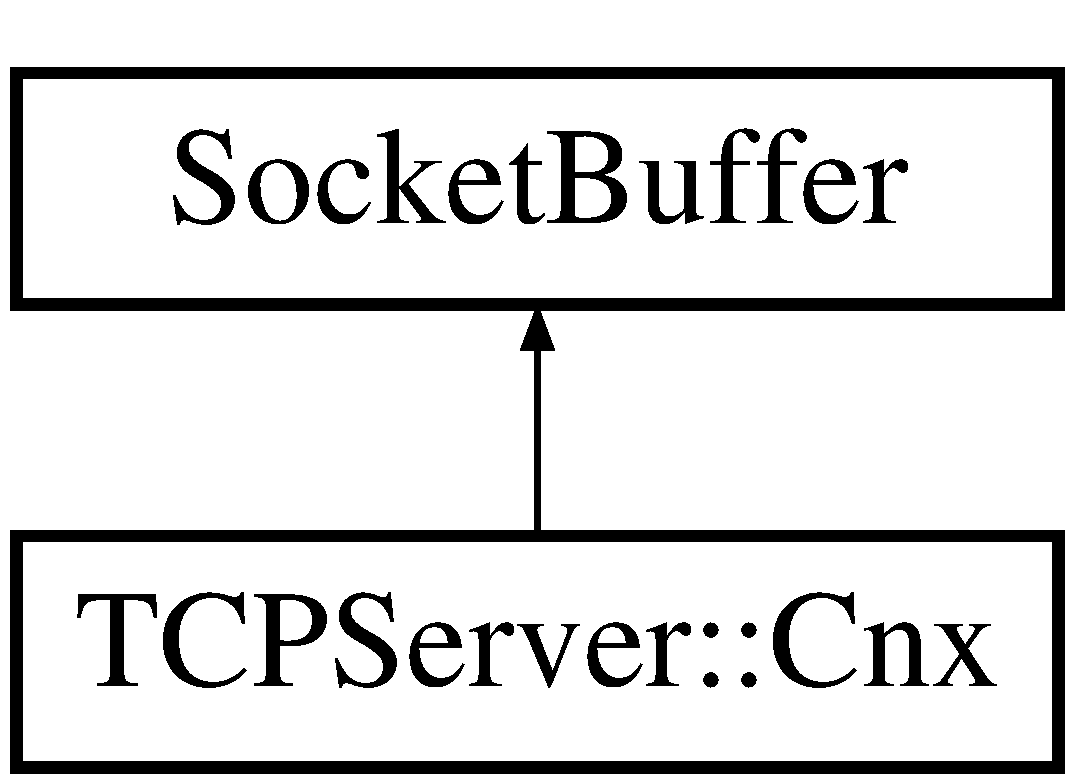
\includegraphics[height=2.000000cm]{class_socket_buffer}
\end{center}
\end{figure}
\subsection*{Public Member Functions}
\begin{DoxyCompactItemize}
\item 
\hypertarget{class_socket_buffer_aa9ed1cc8e166f53606b31246838b3d87}{\hyperlink{class_socket_buffer_aa9ed1cc8e166f53606b31246838b3d87}{Socket\-Buffer} (\hyperlink{class_socket}{Socket} $\ast$socket, size\-\_\-t input\-Buffer\-Size=8192, size\-\_\-t ouput\-Buffer\-Size=8192)}\label{class_socket_buffer_aa9ed1cc8e166f53606b31246838b3d87}

\begin{DoxyCompactList}\small\item\em constructor. The argument must be a valid connected T\-C\-P/\-I\-P \hyperlink{class_socket}{Socket} (i.\-e. of S\-O\-C\-K\-\_\-\-S\-T\-R\-E\-A\-M type) that must N\-O\-T be destructed while this \hyperlink{class_socket_buffer}{Socket\-Buffer} is used. \end{DoxyCompactList}\item 
\hypertarget{class_socket_buffer_a40ad003b90446f69fb0fa4cc18c0d28b}{{\bfseries Socket\-Buffer} (\hyperlink{class_socket}{Socket} \&socket, size\-\_\-t input\-Buffer\-Size=8192, size\-\_\-t ouput\-Buffer\-Size=8192)}\label{class_socket_buffer_a40ad003b90446f69fb0fa4cc18c0d28b}

\item 
\hypertarget{class_socket_buffer_aa9c14ec14e092fc58c4363d2bbc20ffd}{\hyperlink{class_socket}{Socket} $\ast$ {\bfseries socket} ()}\label{class_socket_buffer_aa9c14ec14e092fc58c4363d2bbc20ffd}

\item 
virtual void \hyperlink{class_socket_buffer_ac03353a864ab3a04aa25364a333c0a09}{set\-Separators} (int input\-Separator, int output\-Separator)
\begin{DoxyCompactList}\small\item\em changes the Line Separators. the argument is a character or a negative value (see below)\-: \end{DoxyCompactList}\item 
virtual void \hyperlink{class_socket_buffer_a81a280c639a913b5dbfb12611f339232}{get\-Separators} (int \&input\-Separator, int \&output\-Separator) const 
\begin{DoxyCompactList}\small\item\em returns the Line Separators. \end{DoxyCompactList}\item 
virtual ssize\-\_\-t \hyperlink{class_socket_buffer_a279a372ca946b58455dba0e9c12e213d}{read\-Line} (std\-::string \&str)
\begin{DoxyCompactList}\small\item\em Reads a line of text from a connected socket. The text is stored in the string given as an argument. The other side must send a line of text ended by a Line Separator (. \end{DoxyCompactList}\item 
virtual ssize\-\_\-t \hyperlink{class_socket_buffer_af589c1459da6bca39badf56798c6f859}{write\-Line} (const std\-::string \&str)
\begin{DoxyCompactList}\small\item\em Sends a line of text to a connected socket. Sends the string given as an argument. A Line Separator is automatically added (. \end{DoxyCompactList}\item 
\hypertarget{class_socket_buffer_ab77a4365cfb9625dc996005ffa22bc0c}{virtual ssize\-\_\-t {\bfseries read} (char $\ast$buffer, size\-\_\-t len)}\label{class_socket_buffer_ab77a4365cfb9625dc996005ffa22bc0c}

\item 
\hypertarget{class_socket_buffer_a2ceb624ffd27a27ef500574646c9a8fa}{virtual ssize\-\_\-t {\bfseries write} (const char $\ast$str, size\-\_\-t len)}\label{class_socket_buffer_a2ceb624ffd27a27ef500574646c9a8fa}

\end{DoxyCompactItemize}
\subsection*{Protected Member Functions}
\begin{DoxyCompactItemize}
\item 
\hypertarget{class_socket_buffer_ab2f6ba1d14564967e1714ddd478275d8}{virtual bool {\bfseries retrieve\-Line} (std\-::string \&str, ssize\-\_\-t received)}\label{class_socket_buffer_ab2f6ba1d14564967e1714ddd478275d8}

\end{DoxyCompactItemize}
\subsection*{Protected Attributes}
\begin{DoxyCompactItemize}
\item 
\hypertarget{class_socket_buffer_a19f587689e24a3900a4157be5fa27205}{size\-\_\-t {\bfseries \-\_\-in\-Size}}\label{class_socket_buffer_a19f587689e24a3900a4157be5fa27205}

\item 
\hypertarget{class_socket_buffer_a1ce4a460af7a7fb2f3609bcb9f15ece7}{size\-\_\-t {\bfseries \-\_\-out\-Size}}\label{class_socket_buffer_a1ce4a460af7a7fb2f3609bcb9f15ece7}

\item 
\hypertarget{class_socket_buffer_a8958b13b28d476081c10aac8e25a87d2}{int {\bfseries \-\_\-in\-Sep}}\label{class_socket_buffer_a8958b13b28d476081c10aac8e25a87d2}

\item 
\hypertarget{class_socket_buffer_add088335eb098a067980157b310b22cb}{int {\bfseries \-\_\-out\-Sep}}\label{class_socket_buffer_add088335eb098a067980157b310b22cb}

\item 
\hypertarget{class_socket_buffer_a8575c3a91db81fac18e5634c427faafb}{\hyperlink{class_socket}{Socket} $\ast$ {\bfseries \-\_\-sock}}\label{class_socket_buffer_a8575c3a91db81fac18e5634c427faafb}

\item 
\hypertarget{class_socket_buffer_a8cf67350de772512eff4af7d7f378bed}{struct \hyperlink{struct_input_buffer}{Input\-Buffer} $\ast$ {\bfseries \-\_\-in}}\label{class_socket_buffer_a8cf67350de772512eff4af7d7f378bed}

\end{DoxyCompactItemize}


\subsection{Detailed Description}
Class for exchanging text strings between T\-C\-P/\-I\-P sockets. T\-C\-P/\-I\-P connected sockets do not preserve record boundaries. Messages can be split or merged so that one call to \hyperlink{class_socket_a9275eacdb64056a53cf4b9cf54cd2f1a}{Socket\-::send()} on the sending side does not necessarily correspond to one call to \hyperlink{class_socket_aa5e98b6f2c4e26fcf90d71c8386fc09d}{Socket\-::receive()} on the receiving side. 

The methods of this class solve this problem\-:
\begin{DoxyItemize}
\item by calling \hyperlink{class_socket_a9275eacdb64056a53cf4b9cf54cd2f1a}{Socket\-::send()} or \hyperlink{class_socket_aa5e98b6f2c4e26fcf90d71c8386fc09d}{Socket\-::receive()} as many times as needed
\item by using a Line Separator to separate text lines (\begin{DoxySeeAlso}{See Also}
set\-Separator()) 
\end{DoxySeeAlso}

\end{DoxyItemize}

\subsection{Member Function Documentation}
\hypertarget{class_socket_buffer_a81a280c639a913b5dbfb12611f339232}{\index{Socket\-Buffer@{Socket\-Buffer}!get\-Separators@{get\-Separators}}
\index{get\-Separators@{get\-Separators}!SocketBuffer@{Socket\-Buffer}}
\subsubsection[{get\-Separators}]{\setlength{\rightskip}{0pt plus 5cm}void Socket\-Buffer\-::get\-Separators (
\begin{DoxyParamCaption}
\item[{int \&}]{input\-Separator, }
\item[{int \&}]{output\-Separator}
\end{DoxyParamCaption}
) const\hspace{0.3cm}{\ttfamily [virtual]}}}\label{class_socket_buffer_a81a280c639a913b5dbfb12611f339232}


returns the Line Separators. 

\begin{DoxySeeAlso}{See Also}
\hyperlink{class_socket_buffer_ac03353a864ab3a04aa25364a333c0a09}{set\-Separators()}. 
\end{DoxySeeAlso}
\hypertarget{class_socket_buffer_a279a372ca946b58455dba0e9c12e213d}{\index{Socket\-Buffer@{Socket\-Buffer}!read\-Line@{read\-Line}}
\index{read\-Line@{read\-Line}!SocketBuffer@{Socket\-Buffer}}
\subsubsection[{read\-Line}]{\setlength{\rightskip}{0pt plus 5cm}ssize\-\_\-t Socket\-Buffer\-::read\-Line (
\begin{DoxyParamCaption}
\item[{std\-::string \&}]{str}
\end{DoxyParamCaption}
)\hspace{0.3cm}{\ttfamily [virtual]}}}\label{class_socket_buffer_a279a372ca946b58455dba0e9c12e213d}


Reads a line of text from a connected socket. The text is stored in the string given as an argument. The other side must send a line of text ended by a Line Separator (. 

\begin{DoxySeeAlso}{See Also}
set\-Separator()) which is automatically done by \hyperlink{class_socket_buffer_af589c1459da6bca39badf56798c6f859}{write\-Line()}. The separator is not stored in the argument. 
\end{DoxySeeAlso}
\begin{DoxyReturn}{Returns}
the number of bytes that was received (including the separator) except if\-:
\begin{DoxyItemize}
\item shutdown\-Output() was called on the other side (0 is returned)
\item an error occured (Socket\-::\-Failed is returned)
\item the socket is invalid (Socket\-::\-Invalid\-Socket is returned) 
\end{DoxyItemize}
\end{DoxyReturn}
\begin{DoxyNote}{Note}
this method may block. 
\end{DoxyNote}
\hypertarget{class_socket_buffer_ac03353a864ab3a04aa25364a333c0a09}{\index{Socket\-Buffer@{Socket\-Buffer}!set\-Separators@{set\-Separators}}
\index{set\-Separators@{set\-Separators}!SocketBuffer@{Socket\-Buffer}}
\subsubsection[{set\-Separators}]{\setlength{\rightskip}{0pt plus 5cm}void Socket\-Buffer\-::set\-Separators (
\begin{DoxyParamCaption}
\item[{int}]{input\-Separator, }
\item[{int}]{output\-Separator}
\end{DoxyParamCaption}
)\hspace{0.3cm}{\ttfamily [virtual]}}}\label{class_socket_buffer_ac03353a864ab3a04aa25364a333c0a09}


changes the Line Separators. the argument is a character or a negative value (see below)\-: 


\begin{DoxyItemize}
\item if {\itshape input\-Separator} is $<$ 0 (the default) a line is considered to be terminated by any one of '\par
' or '' or '\par
' followed by ''
\item if {\itshape output\-Separator} is $<$ 0 a line is terminated by '\par
' followed by ''. The default value is '\par
'. 
\end{DoxyItemize}\hypertarget{class_socket_buffer_af589c1459da6bca39badf56798c6f859}{\index{Socket\-Buffer@{Socket\-Buffer}!write\-Line@{write\-Line}}
\index{write\-Line@{write\-Line}!SocketBuffer@{Socket\-Buffer}}
\subsubsection[{write\-Line}]{\setlength{\rightskip}{0pt plus 5cm}ssize\-\_\-t Socket\-Buffer\-::write\-Line (
\begin{DoxyParamCaption}
\item[{const std\-::string \&}]{str}
\end{DoxyParamCaption}
)\hspace{0.3cm}{\ttfamily [virtual]}}}\label{class_socket_buffer_af589c1459da6bca39badf56798c6f859}


Sends a line of text to a connected socket. Sends the string given as an argument. A Line Separator is automatically added (. 

\begin{DoxySeeAlso}{See Also}
set\-Separator()). 
\end{DoxySeeAlso}
\begin{DoxyReturn}{Returns}
the number of bytes that was sent (including the separator) except if\-:
\begin{DoxyItemize}
\item shutdown\-Input() was called on the other side (0 is returned)
\item an error occured (Socket\-::\-Failed is returned)
\item the socket is invalid (Socket\-::\-Invalid\-Socket is returned) 
\end{DoxyItemize}
\end{DoxyReturn}
\begin{DoxyNote}{Note}
this method may block. 
\end{DoxyNote}


The documentation for this class was generated from the following files\-:\begin{DoxyCompactItemize}
\item 
Socket.\-h\item 
Socket.\-cpp\end{DoxyCompactItemize}

\hypertarget{class_t_c_p_server}{\section{T\-C\-P\-Server Class Reference}
\label{class_t_c_p_server}\index{T\-C\-P\-Server@{T\-C\-P\-Server}}
}


T\-C\-P/\-I\-P I\-Pv4 server. The server supports T\-C\-P/\-I\-P A\-F\-\_\-\-I\-N\-E\-T connections (following the I\-Pv4 Internet protocol) with multiple clients. One thread is used per client.  




{\ttfamily \#include $<$T\-C\-P\-Server.\-h$>$}

\subsection*{Classes}
\begin{DoxyCompactItemize}
\item 
class \hyperlink{class_t_c_p_server_1_1_callback}{Callback}
\item 
class \hyperlink{class_t_c_p_server_1_1_callback_impl}{Callback\-Impl}
\item 
class \hyperlink{class_t_c_p_server_1_1_cnx}{Cnx}
\begin{DoxyCompactList}\small\item\em represents a connection with a given client. \end{DoxyCompactList}\item 
class \hyperlink{class_t_c_p_server_1_1_lock}{Lock}
\begin{DoxyCompactList}\small\item\em locks the server in read mode or in write mode. In order to avoid concurrency problems between threads, the callback method that processes requests should instantiate a \hyperlink{class_t_c_p_server_1_1_lock}{Lock} object in the stack. The \hyperlink{class_t_c_p_server_1_1_lock}{Lock} must be instantiated in write mode if the request changes data, or in read mode otherwise. A write lock blocks all other locks (hence, all other threads) until the callback method that issued the write lock returns. \end{DoxyCompactList}\end{DoxyCompactItemize}
\subsection*{Public Member Functions}
\begin{DoxyCompactItemize}
\item 
\hypertarget{class_t_c_p_server_a3a5e3cfe42c676ed71f2bc58dcc92bda}{\hyperlink{class_t_c_p_server_a3a5e3cfe42c676ed71f2bc58dcc92bda}{T\-C\-P\-Server} ()}\label{class_t_c_p_server_a3a5e3cfe42c676ed71f2bc58dcc92bda}

\begin{DoxyCompactList}\small\item\em constructor\-: initializes the \hyperlink{class_t_c_p_server}{T\-C\-P\-Server}. \end{DoxyCompactList}\item 
\hypertarget{class_t_c_p_server_abc497ac52355e53986a6a1bd1acb9581}{virtual \hyperlink{class_t_c_p_server_abc497ac52355e53986a6a1bd1acb9581}{$\sim$\-T\-C\-P\-Server} ()}\label{class_t_c_p_server_abc497ac52355e53986a6a1bd1acb9581}

\begin{DoxyCompactList}\small\item\em destructor\-: cleans up the \hyperlink{class_t_c_p_server}{T\-C\-P\-Server}. \end{DoxyCompactList}\item 
virtual int \hyperlink{class_t_c_p_server_a1409041961e91f1dbc4933483b4c3b23}{run} (int port)
\begin{DoxyCompactList}\small\item\em starts the main loop of the server on this port. This function binds an internal \hyperlink{class_server_socket}{Server\-Socket} then starts an infinite main loop that receives requests from clients. The function creates one thread per client. \end{DoxyCompactList}\item 
{\footnotesize template$<$class T $>$ }\\void \hyperlink{class_t_c_p_server_ac62c8c7a1d1137b74e2a1fa6d8a4a876}{set\-Callback} (T $\ast$obj, bool(T\-::$\ast$func)(\hyperlink{class_t_c_p_server_1_1_cnx}{Cnx} \&, const std\-::string \&request, std\-::string \&response))
\begin{DoxyCompactList}\small\item\em changes the callback method that processes requests. The first argument must be an object, the second argument a method of this object. This method will be called each time the \hyperlink{class_t_c_p_server}{T\-C\-P\-Server} receives a 'request' from a client in order to perform a computation and return a 'response' to this client. \end{DoxyCompactList}\end{DoxyCompactItemize}
\subsection*{Protected Member Functions}
\begin{DoxyCompactItemize}
\item 
\hypertarget{class_t_c_p_server_af99977f3ec05210e91d02aa9c693254b}{virtual void \hyperlink{class_t_c_p_server_af99977f3ec05210e91d02aa9c693254b}{read\-Messages} (\hyperlink{class_t_c_p_server_1_1_cnx}{T\-C\-P\-Server\-::\-Cnx} $\ast$)}\label{class_t_c_p_server_af99977f3ec05210e91d02aa9c693254b}

\begin{DoxyCompactList}\small\item\em reads messages from a given client on the corresponding thread. \end{DoxyCompactList}\item 
\hypertarget{class_t_c_p_server_a2f053dfc720aab308f97ccc8a789adc4}{virtual void \hyperlink{class_t_c_p_server_a2f053dfc720aab308f97ccc8a789adc4}{print\-Msg} (const std\-::string \&msg, const \hyperlink{class_t_c_p_server_1_1_cnx}{T\-C\-P\-Server\-::\-Cnx} $\ast$=0)}\label{class_t_c_p_server_a2f053dfc720aab308f97ccc8a789adc4}

\begin{DoxyCompactList}\small\item\em prints warning and error messages on the terminal. \end{DoxyCompactList}\end{DoxyCompactItemize}
\subsection*{Protected Attributes}
\begin{DoxyCompactItemize}
\item 
\hypertarget{class_t_c_p_server_a9c2891cf40b19735bceb22605a5e867e}{\hyperlink{class_server_socket}{Server\-Socket} {\bfseries \-\_\-servsock}}\label{class_t_c_p_server_a9c2891cf40b19735bceb22605a5e867e}

\item 
\hypertarget{class_t_c_p_server_a1f7a87b1f42950325d005c8a0ca9427e}{std\-::shared\-\_\-ptr$<$ \hyperlink{class_t_c_p_server_1_1_callback}{Callback} $>$ {\bfseries \-\_\-callback}}\label{class_t_c_p_server_a1f7a87b1f42950325d005c8a0ca9427e}

\item 
\hypertarget{class_t_c_p_server_a130152438b313a1c4470c842a063257d}{pthread\-\_\-rwlock\-\_\-t {\bfseries \-\_\-threadlock}}\label{class_t_c_p_server_a130152438b313a1c4470c842a063257d}

\end{DoxyCompactItemize}


\subsection{Detailed Description}
T\-C\-P/\-I\-P I\-Pv4 server. The server supports T\-C\-P/\-I\-P A\-F\-\_\-\-I\-N\-E\-T connections (following the I\-Pv4 Internet protocol) with multiple clients. One thread is used per client. 

The \hyperlink{class_t_c_p_server_a1409041961e91f1dbc4933483b4c3b23}{run()} method binds an internal \hyperlink{class_server_socket}{Server\-Socket} then starts an infinite main loop that receives requests from clients. Requests can be received concurrently thanks to threads.

A callback method is called each time the sever receives a request from a client (\begin{DoxySeeAlso}{See Also}
\hyperlink{class_t_c_p_server_ac62c8c7a1d1137b74e2a1fa6d8a4a876}{set\-Callback()} to set this method). This method can issue read and write locks to avoid concurrency issues (

\hyperlink{class_t_c_p_server_1_1_lock}{Lock}). 
\end{DoxySeeAlso}


\subsection{Member Function Documentation}
\hypertarget{class_t_c_p_server_a1409041961e91f1dbc4933483b4c3b23}{\index{T\-C\-P\-Server@{T\-C\-P\-Server}!run@{run}}
\index{run@{run}!TCPServer@{T\-C\-P\-Server}}
\subsubsection[{run}]{\setlength{\rightskip}{0pt plus 5cm}int T\-C\-P\-Server\-::run (
\begin{DoxyParamCaption}
\item[{int}]{port}
\end{DoxyParamCaption}
)\hspace{0.3cm}{\ttfamily [virtual]}}}\label{class_t_c_p_server_a1409041961e91f1dbc4933483b4c3b23}


starts the main loop of the server on this port. This function binds an internal \hyperlink{class_server_socket}{Server\-Socket} then starts an infinite main loop that receives requests from clients. The function creates one thread per client. 

\begin{DoxyReturn}{Returns}
0 on normal termination or a negative value if the \hyperlink{class_server_socket}{Server\-Socket} could not be bound (value is then one of \hyperlink{class_socket_a9f68308228badcdd299cd83e62e36976}{Socket\-::\-Errors}). 
\end{DoxyReturn}
\hypertarget{class_t_c_p_server_ac62c8c7a1d1137b74e2a1fa6d8a4a876}{\index{T\-C\-P\-Server@{T\-C\-P\-Server}!set\-Callback@{set\-Callback}}
\index{set\-Callback@{set\-Callback}!TCPServer@{T\-C\-P\-Server}}
\subsubsection[{set\-Callback}]{\setlength{\rightskip}{0pt plus 5cm}template$<$class T $>$ void T\-C\-P\-Server\-::set\-Callback (
\begin{DoxyParamCaption}
\item[{T $\ast$}]{obj, }
\item[{bool(T\-::$\ast$)({\bf Cnx} \&, const std\-::string \&request, std\-::string \&response)}]{func}
\end{DoxyParamCaption}
)\hspace{0.3cm}{\ttfamily [inline]}}}\label{class_t_c_p_server_ac62c8c7a1d1137b74e2a1fa6d8a4a876}


changes the callback method that processes requests. The first argument must be an object, the second argument a method of this object. This method will be called each time the \hyperlink{class_t_c_p_server}{T\-C\-P\-Server} receives a 'request' from a client in order to perform a computation and return a 'response' to this client. 

Arguments and return value of the method\-:
\begin{DoxyItemize}
\item the 'request' and the 'response' are provided through the corresponding parameters of the method.
\item the connection with the client will be closed if the method returns false 
\end{DoxyItemize}

The documentation for this class was generated from the following files\-:\begin{DoxyCompactItemize}
\item 
T\-C\-P\-Server.\-h\item 
T\-C\-P\-Server.\-cpp\end{DoxyCompactItemize}

\hypertarget{class_video}{\section{Video Class Reference}
\label{class_video}\index{Video@{Video}}
}
Inheritance diagram for Video\-:\begin{figure}[H]
\begin{center}
\leavevmode
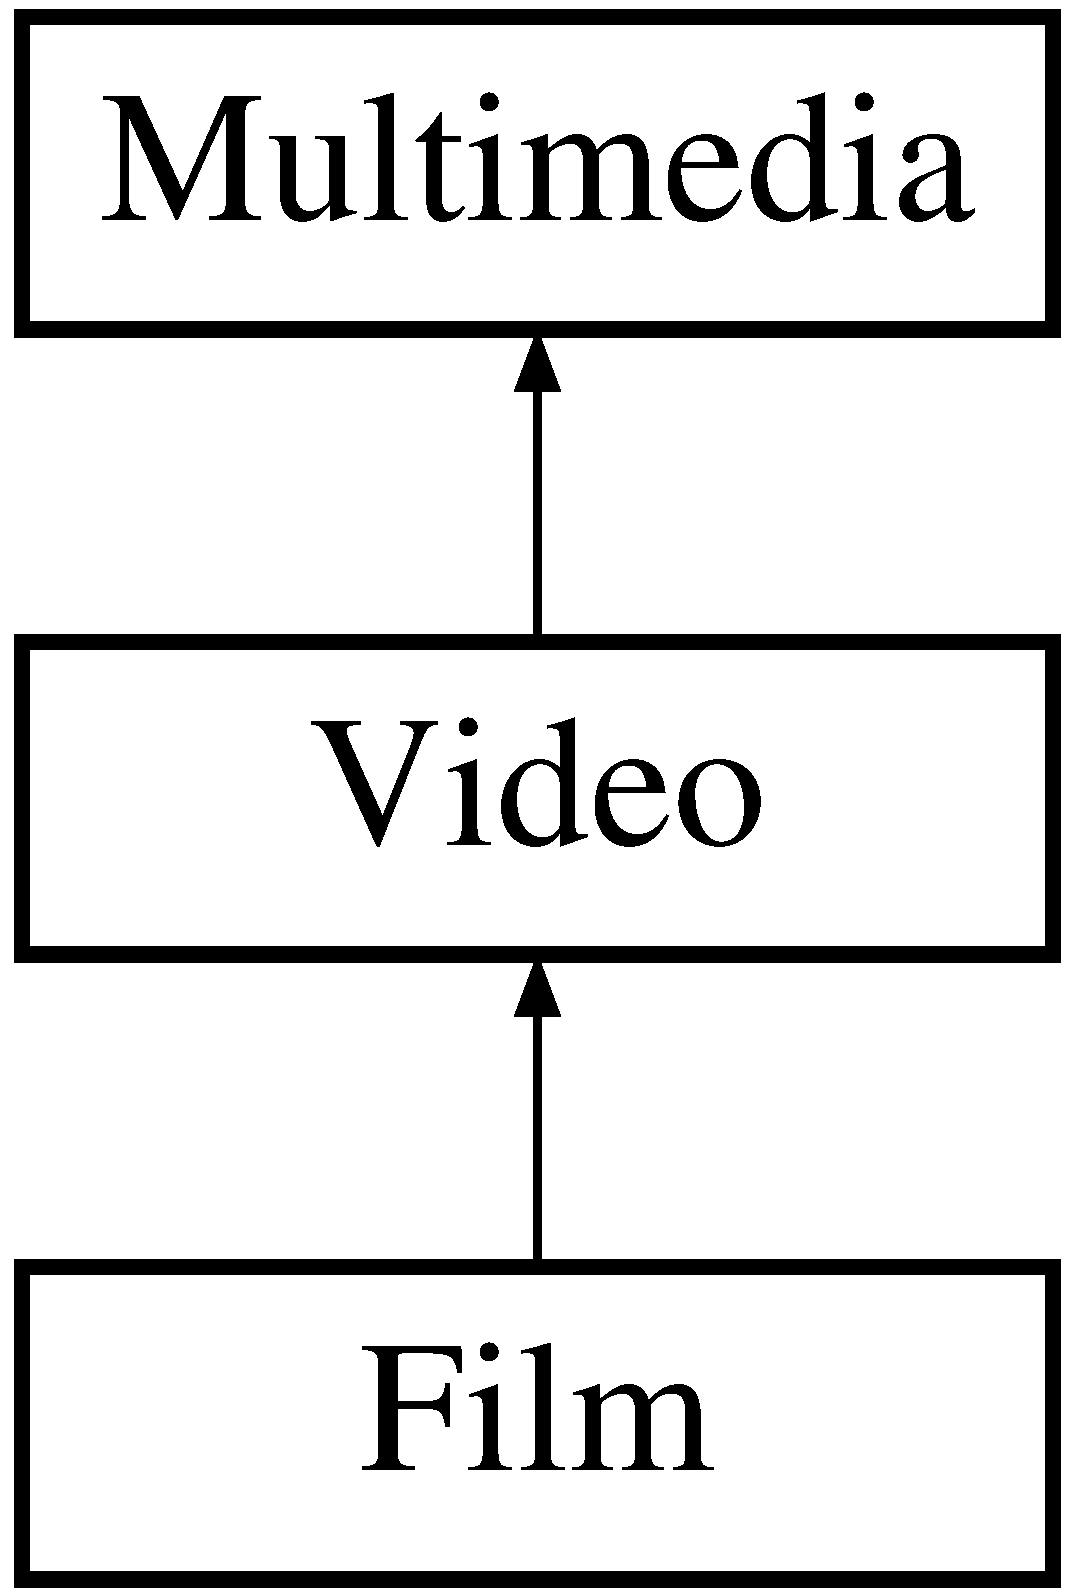
\includegraphics[height=3.000000cm]{class_video}
\end{center}
\end{figure}
\subsection*{Public Member Functions}
\begin{DoxyCompactItemize}
\item 
\hypertarget{class_video_a19f29b0c0efae6ce7a89f1ae61f81f70}{{\bfseries Video} (int delay=0)}\label{class_video_a19f29b0c0efae6ce7a89f1ae61f81f70}

\item 
\hypertarget{class_video_ae748826e2e68c45a2030258042832d08}{{\bfseries Video} (const std\-::string \&name, const std\-::string \&path, int delay=0)}\label{class_video_ae748826e2e68c45a2030258042832d08}

\item 
\hypertarget{class_video_a1bd10186658fb7399508bd43c3dc6c51}{virtual std\-::ostream \& \hyperlink{class_video_a1bd10186658fb7399508bd43c3dc6c51}{print} (std\-::ostream \&oss) const }\label{class_video_a1bd10186658fb7399508bd43c3dc6c51}

\begin{DoxyCompactList}\small\item\em Redefinition of print method allowing child redefinition too. \end{DoxyCompactList}\item 
\hypertarget{class_video_a591c7d2a74b0095373b5df4e20f38203}{virtual void \hyperlink{class_video_a591c7d2a74b0095373b5df4e20f38203}{execute} () const }\label{class_video_a591c7d2a74b0095373b5df4e20f38203}

\begin{DoxyCompactList}\small\item\em Open the video inside Unix environment (doesn't work within windows if no unix environment with mpv command is installed) \end{DoxyCompactList}\item 
\hypertarget{class_video_af4590349144352c253de21701d20c8fc}{void {\bfseries set\-Delay} (int delay)}\label{class_video_af4590349144352c253de21701d20c8fc}

\item 
\hypertarget{class_video_a0585044752fbca505f0f00ced0d535af}{int {\bfseries get\-Delay} () const }\label{class_video_a0585044752fbca505f0f00ced0d535af}

\end{DoxyCompactItemize}
\subsection*{Protected Attributes}
\begin{DoxyCompactItemize}
\item 
\hypertarget{class_video_a6ee93d1d2241dede568773d78547de64}{int {\bfseries delay}}\label{class_video_a6ee93d1d2241dede568773d78547de64}

\end{DoxyCompactItemize}


The documentation for this class was generated from the following files\-:\begin{DoxyCompactItemize}
\item 
Video.\-hpp\item 
Video.\-cpp\end{DoxyCompactItemize}

%--- End generated contents ---

% Index
\newpage
\phantomsection
\addcontentsline{toc}{chapter}{Index}
\printindex

\end{document}
